\documentclass[11pt,a4paper]{article}

\usepackage[utf8]{inputenc}
\usepackage[T1]{fontenc}
\usepackage[spanish,es-tabla,es-nodecimaldot]{babel}
\usepackage{lmodern}
\usepackage[margin=2.5cm]{geometry}
\usepackage{amsmath}
\usepackage{amssymb}
\usepackage{graphicx}
\usepackage{booktabs}
\usepackage{array}
\usepackage{float}
\usepackage{subcaption}
\usepackage{tikz}
\usetikzlibrary{positioning,arrows.meta,fit}
\usepackage[authoryear,round]{natbib}
\usepackage{hyperref}
\hypersetup{colorlinks=true,linkcolor=black,citecolor=black,urlcolor=blue}

\graphicspath{{figuras/}}
\setlength{\emergencystretch}{3em}

% Todas las citas del informe van en negrita
\AtBeginDocument{%
  \let\citepOriginal\citep
  \renewcommand*{\citep}[1]{\textbf{\citepOriginal{#1}}}%
  \let\citetOriginal\citet
  \renewcommand*{\citet}[1]{\textbf{\citetOriginal{#1}}}%
  \let\citealpOriginal\citealp
  \renewcommand*{\citealp}[1]{\textbf{\citealpOriginal{#1}}}%
}

\begin{document}

\begin{titlepage}
\centering
{\large Universidad Nacional de Costa Rica\par}
{\large Escuela de Informática\par}
{\large EIF420O Inteligencia Artificial\par}
\vspace{4cm}
{\LARGE\bfseries Laboratorio 03\par}
\vspace{0.5cm}
{\Large Métodos supervisados: regresión y benchmarking con modelos lineales, SVR y árboles\par}
\vspace{4cm}
{\large Brandon Brenes Umaña -- 119180779\par}
{\large Sebastián Alpízar Porras -- 118240079\par}
{\large Darío Gutiérrez Jiménez -- 119360478\par}
\vspace{2cm}
{\large Profesor: Dr. Juan Murillo-Morera\par}
\vfill
{\large II Ciclo 2026\par}
\end{titlepage}

\tableofcontents
\newpage
% ======================================================================
\section{Introducción}

En el Laboratorio 02 trabajamos con clasificación, donde la variable a predecir es una categoría. En este laboratorio pasamos a la otra tarea supervisada, la \textit{regresión}, en la que la variable a predecir es numérica y continua, y el modelo debe estimar su valor y no solo una clase \citep{james2013,hastie2009}. Además de entrenar modelos, el laboratorio pide hacer un \textit{benchmarking}: comparar de forma sistemática algoritmos de una misma familia y de familias distintas, con las mismas condiciones experimentales, y justificar cuáles son los mejores \citep{hothorn2005}.

Escogimos el conjunto de datos \textbf{Communities and Crime} de \citet{redmond2002}, que ya usamos en el Laboratorio 01 con métodos no supervisados. Describe 1994 comunidades de Estados Unidos con 100 variables socioeconómicas, demográficas y policiales, y la variable a predecir es la tasa de crímenes violentos por habitante. Es un problema de regresión clásico: la respuesta es continua, hay muchas predictoras, todas numéricas y sin valores faltantes, y muchas de ellas están muy correlacionadas entre sí, lo que permite ver para qué sirven la regularización de Lasso y Ridge.

Trabajamos con tres familias de algoritmos: los modelos \textbf{lineales} (regresión lineal simple y múltiple, Lasso, LassoCV, Ridge y RidgeCV), las \textbf{máquinas de vectores de soporte} para regresión (SVR, con kernels rbf, lineal y polinomial) y los \textbf{árboles} (árbol de decisión, Random Forest y, como extra, XGBoost). Para cada algoritmo corrimos la configuración estándar y varias variaciones, escogimos el mejor modelo, comparamos los algoritmos dentro de cada familia y luego entre familias. Como un solo conjunto de prueba puede favorecer a un modelo por azar, terminamos con una validación cruzada repetida y pruebas estadísticas para decidir si las diferencias entre los mejores modelos son reales \citep{demsar2006}. Todo se integró al framework del curso, con una nueva clase \texttt{Regresion} que hereda de \texttt{Supervisado} \citep{pedregosa2011}.

% ======================================================================
\section{Definiciones y conceptos}

\subsection{Regresión supervisada}
Igual que en clasificación, se tiene un conjunto de individuos descritos por predictoras $X=(X_1,\dots,X_p)$ y una variable a predecir $Y$, pero ahora $Y\in\mathbb{R}$. Se busca una función $\hat f$ tal que $\hat y=\hat f(x)$ esté lo más cerca posible del valor real en individuos que el modelo no vio \citep{james2013}. El error de un modelo en datos nuevos se descompone en sesgo, varianza y ruido irreducible: los modelos muy simples tienen mucho sesgo (no captan la relación), los muy flexibles tienen mucha varianza (memorizan el entrenamiento), y ningún modelo puede bajar del ruido propio de los datos \citep{hastie2009}. Por eso los datos se dividen en entrenamiento y prueba, y los hiperparámetros se escogen con validación cruzada.

\subsection{Regresión lineal simple y múltiple}
La regresión lineal supone que $Y$ es una combinación lineal de las predictoras más un error:
\[
\hat y = w_0 + w_1x_1+\dots+w_px_p ,
\]
y estima los coeficientes por \textbf{mínimos cuadrados ordinarios} (MCO), es decir, minimizando la suma de los residuos al cuadrado $\sum_i (y_i-\hat y_i)^2$ \citep{james2013}. En la regresión \textit{simple} hay una sola predictora ($p=1$) y el modelo es una recta; en la \textit{múltiple} se usan todas. Cada coeficiente $w_j$ indica cuánto cambia $\hat y$ cuando $x_j$ aumenta una unidad y las demás se mantienen fijas. Cuando las predictoras están muy correlacionadas entre sí (\textit{multicolinealidad}), esa interpretación deja de tener sentido: los coeficientes se vuelven inestables, pueden tener el signo contrario al esperado y su varianza crece mucho \citep{dormann2013}.

\subsection{Regularización: Ridge y Lasso}
La regularización agrega a los mínimos cuadrados una penalización por el tamaño de los coeficientes, controlada por un hiperparámetro $\alpha\ge0$. \textbf{Ridge} \citep{hoerl1970} usa la norma L2 y \textbf{Lasso} \citep{tibshirani1996} la norma L1:
\[
\text{Ridge: }\min_w \sum_i (y_i-\hat y_i)^2+\alpha\sum_j w_j^2 ,\qquad
\text{Lasso: }\min_w \frac{1}{2n}\sum_i (y_i-\hat y_i)^2+\alpha\sum_j |w_j| .
\]
Con $\alpha=0$ las dos son MCO, y al crecer $\alpha$ los coeficientes se encogen hacia cero, lo que aumenta un poco el sesgo pero baja la varianza. Ridge encoge todos los coeficientes sin anular ninguno y reparte el peso entre las variables correlacionadas. Lasso, por la forma de la norma L1, lleva muchos coeficientes exactamente a cero, así que además \textit{selecciona variables}. Cuando hay grupos de variables muy correlacionadas, Lasso tiende a quedarse con una sola de cada grupo de forma algo arbitraria \citep{zou2005}. Como la penalización depende de la escala de los coeficientes, normalmente se estandarizan las predictoras antes de ajustar. \textbf{LassoCV} y \textbf{RidgeCV} escogen $\alpha$ automáticamente con validación cruzada sobre el entrenamiento: prueban una rejilla de valores, se quedan con el de menor error y reajustan el modelo con todo el entrenamiento. RidgeCV, por defecto, usa validación cruzada dejando uno fuera, que en Ridge tiene una fórmula cerrada y es muy rápida \citep{hastie2009}.

\subsection{Regresión con máquinas de vectores de soporte (SVR)}
SVR \citep{drucker1997,smola2004} busca una función lo más ``plana'' posible que se equivoque a lo sumo $\varepsilon$ en cada individuo. Los errores menores que $\varepsilon$ no se penalizan (pérdida $\varepsilon$-insensible) y los mayores se penalizan linealmente con un peso $C$:
\[
\min_{w,b}\ \tfrac12\lVert w\rVert^2 + C\sum_i \max\big(0,\ |y_i-\hat y_i|-\varepsilon\big).
\]
La solución depende solo de los \textit{vectores de soporte}, los individuos que quedan fuera del tubo de ancho $\varepsilon$. Con el \textit{truco del kernel}, SVR ajusta funciones no lineales: el kernel lineal da un modelo lineal, el polinomial $(\gamma\,x^\top z+r)^d$ incluye interacciones de grado $d$, y el rbf $\exp(-\gamma\lVert x-z\rVert^2)$ produce una función suave cuya flexibilidad depende de $\gamma$ \citep{smola2004}. $C$ grande permite ajustarse mucho a los datos (riesgo de sobreajuste), $\varepsilon$ grande hace el modelo más tolerante y $\gamma$ grande vuelve local a cada vector de soporte. Como usa distancias y productos punto, las variables se deben estandarizar.

\subsection{Árboles de regresión, Random Forest y XGBoost}
Un \textbf{árbol de regresión} \citep{breiman1984} divide los datos con preguntas del tipo ``¿$x_j\le c$?'' y predice en cada hoja el promedio de $Y$ de los individuos que caen en ella. En cada nodo escoge la división que más reduce el error cuadrático. Sin límites crece hasta memorizar el entrenamiento, así que se controla con la profundidad (\texttt{max\_depth}), el mínimo de individuos por hoja (\texttt{min\_samples\_leaf}) o la poda por costo-complejidad (\texttt{ccp\_alpha}). Su predicción es una función escalonada.

\textbf{Random Forest} \citep{breiman2001} promedia muchos árboles entrenados con muestras bootstrap, considerando en cada división solo un subconjunto aleatorio de variables (\texttt{max\_features}). En regresión, \citet{breiman2001} recomienda usar $p/3$ variables; en scikit-learn el valor por defecto es usar todas, que equivale a \textit{bagging} puro \citep{probst2019}. Promediar árboles poco correlacionados baja la varianza.

\textbf{XGBoost} \citep{chen2016} es \textit{gradient boosting} \citep{friedman2001}: agrega árboles pequeños en secuencia, cada uno ajustado a los residuos de los anteriores, multiplicados por una tasa de aprendizaje, y con una penalización por la complejidad de los árboles. No es obligatorio en este laboratorio, pero lo incluimos porque el código guía del curso usa potenciación y el framework ya lo tenía del Laboratorio 02.

\subsection{Índices de calidad para regresión}
Con $e_i=y_i-\hat y_i$ el error de cada individuo de prueba, usamos los tres índices del código guía del curso más el $R^2$:
\[
\text{RMSE}=\sqrt{\tfrac1n\textstyle\sum_i e_i^2},\qquad
\text{MAE}=\tfrac1n\textstyle\sum_i |e_i|,\qquad
\text{ER}=\dfrac{\sum_i|e_i|}{\sum_i|y_i|},\qquad
R^2=1-\dfrac{\sum_i e_i^2}{\sum_i (y_i-\bar y)^2}.
\]
El RMSE y el MAE están en las unidades de $Y$. El RMSE castiga más los errores grandes y el MAE es más robusto a valores atípicos \citep{willmott2005,chai2014}. El error relativo (ER) expresa el error absoluto total como proporción del total de la variable. El $R^2$ es la proporción de la varianza de $Y$ que explica el modelo: 1 es perfecto, 0 equivale a predecir siempre el promedio y puede ser negativo si el modelo es peor que eso. Usamos el \textbf{RMSE} como criterio para escoger el mejor modelo de cada algoritmo, porque es la raíz de la función que minimizan casi todos los modelos, y los demás índices como apoyo. También analizamos los \textbf{residuos}: si un modelo está bien especificado, los residuos no deberían tener estructura respecto a la predicción.

\subsection{Benchmarking y pruebas estadísticas}
Un \textit{benchmarking} compara algoritmos bajo un diseño experimental controlado: los mismos datos, las mismas particiones y los mismos índices \citep{hothorn2005}. Comparamos de dos formas. Primero, dentro de cada familia y entre familias con el conjunto de prueba. Segundo, con una \textbf{validación cruzada de 10 particiones repetida 3 veces} sobre el entrenamiento, en la que todos los modelos usan exactamente las mismas 30 particiones, de modo que se pueden comparar en pares \citep{kohavi1995}. Sobre esos resultados aplicamos la \textbf{prueba de Friedman} \citep{friedman1937}, que ordena los modelos en cada partición y prueba si sus rangos promedio difieren, y luego la \textbf{prueba de rangos con signo de Wilcoxon} \citep{wilcoxon1945} entre el mejor modelo y cada uno de los demás, corrigiendo los valores $p$ por comparaciones múltiples con el método de \citet{holm1979}. Son pruebas no paramétricas, como recomienda \citet{demsar2006} para comparar algoritmos. Hay que tener presente una limitación: las particiones de una validación cruzada comparten individuos, así que no son del todo independientes, y las pruebas tienden a encontrar diferencias significativas con más facilidad de lo que deberían \citep{dietterich1998,nadeau2003}. Por eso las usamos como apoyo y no como única evidencia.
% ======================================================================
\section{Mapa conceptual}

El mapa continúa el de los laboratorios anteriores. Siguiendo a \citet{james2013}, los métodos supervisados se dividen según el tipo de variable a predecir: la clasificación (Laboratorio 02) cuando es categórica y la regresión (este laboratorio) cuando es continua. La parte de regresión se organiza en las tres familias que comparamos. Todas comparten el mismo preprocesamiento, los mismos índices de calidad y el mismo protocolo de benchmarking, que es lo que permite compararlas de forma justa \citep{hothorn2005}.

\begin{figure}[H]
\centering
\resizebox{\textwidth}{!}{%
\begin{tikzpicture}[
  every node/.style={draw,rounded corners,align=center,font=\small},
  n0/.style={fill=gray!40,font=\Large\bfseries},
  n1/.style={fill=gray!20,font=\bfseries},
  n2/.style={fill=blue!10},
  n3/.style={fill=orange!15},
  n4/.style={draw=gray,font=\footnotesize,text width=3.7cm},
  n5/.style={fill=green!10,text width=17cm},
  vie/.style={fill=gray!8,draw=gray,font=\footnotesize,text width=4.2cm},
  et/.style={draw=none,font=\itshape\small,text=gray},
  -{Stealth},thick]
% ---------------- Raíz y laboratorios anteriores ----------------
\node[n0] (raiz) at (0,0) {Aprendizaje automático};
\node[n2] (eda) at (0,1.2) {EDA: nulos, duplicados, outliers, correlación, estandarizar};
\draw (eda) -- (raiz);
\node[vie] (ns) at (-7.5,-0.6) {\textbf{Métodos no supervisados} (Laboratorio 1): ACP, t-SNE, UMAP, K-means, HAC};
\node[n1] (sup) at (0,-2) {Métodos supervisados};
\draw (raiz) -- (ns);
\draw (raiz) -- (sup);
\node[vie] (cla) at (7.5,-2.6) {\textbf{Clasificación} (Laboratorio 2): $Y$ categórica; KNN, DT, RF, XGBoost, AdaBoost; matriz de confusión, F1, AUC};
\node[n1] (reg) at (0,-3.9) {Regresión\\($Y$ continua)};
\node[et,left=0.3cm of reg] {(Laboratorio 3)};
\draw (sup) -- (cla);
\draw (sup) -- (reg);
% ---------------- Preparación ----------------
\node[n5] (pre) at (0,-5.9) {\textbf{Preparación}: excluir variables que no son predictoras; partición aleatoria 75/25 con semilla fija; imputación; estandarización (penalizados y SVR); \texttt{SelectKBest} con $F$ de regresión; todo dentro de un \texttt{Pipeline} para evitar fuga de información};
\draw (reg) -- (pre);
% ---------------- Familias ----------------
\node[n2] (lin) at (-6.6,-8) {Familia lineal};
\node[n2] (ker) at (0,-8) {Familia de núcleos};
\node[n2] (arb) at (6.6,-8) {Familia de árboles};
\draw (pre) -- (lin); \draw (pre) -- (ker); \draw (pre) -- (arb);
\node[n3] (mco) at (-8.8,-9.8) {MCO: lineal\\simple y múltiple};
\node[n3] (pen) at (-4.4,-9.8) {Penalizados:\\Lasso (L1), Ridge (L2)};
\node[n3] (svr) at (0,-9.8) {SVR (kernels rbf,\\lineal, polinomial)};
\node[n3] (dt) at (4.4,-9.8) {Árbol de\\regresión (DT)};
\node[n3] (ens) at (8.8,-9.8) {Ensambles: RF\\(\textit{bagging}), XGBoost};
\draw (lin) -- (mco); \draw (lin) -- (pen);
\draw (ker) -- (svr);
\draw (arb) -- (dt); \draw (arb) -- (ens);
\node[n4,anchor=north] (d1) at (-8.8,-10.9) {minimiza $\sum e_i^2$; coeficientes interpretables; inestable con multicolinealidad};
\node[n4,anchor=north] (d2) at (-4.4,-10.9) {$\alpha$ encoge los coeficientes; Lasso los anula (selecciona variables); LassoCV y RidgeCV escogen $\alpha$ por validación cruzada};
\node[n4,anchor=north] (d3) at (0,-10.9) {pérdida $\varepsilon$-insensible; $C$, $\varepsilon$, $\gamma$; vectores de soporte; necesita escalar};
\node[n4,anchor=north] (d4) at (4.4,-10.9) {divisiones que bajan el error cuadrático; profundidad, hojas mínimas, poda; predicción escalonada};
\node[n4,anchor=north] (d5) at (8.8,-10.9) {RF: promedio de árboles, \texttt{max\_features}; XGBoost: árboles en secuencia sobre los residuos};
\draw (mco) -- (d1); \draw (pen) -- (d2); \draw (svr) -- (d3); \draw (dt) -- (d4); \draw (ens) -- (d5);
\draw[dashed,blue] (mco.east) -- node[draw=none,above,font=\scriptsize]{$\alpha=0$} (pen.west);
\draw[dashed,blue] (dt.east) -- node[draw=none,above,font=\scriptsize]{árbol base} (ens.west);
% ---------------- Evaluación y benchmarking ----------------
\node[n5] (ev) at (0,-14.6) {\textbf{Evaluación}: RMSE (criterio de selección), MAE, error relativo (ER) y $R^2$; gráfico de valores reales contra predicciones; análisis de residuos; coeficientes e importancia de variables};
\node[n5] (bm) at (0,-16.3) {\textbf{Benchmarking}: (1) dentro de cada familia, (2) entre familias con el mejor modelo de cada algoritmo; validación cruzada $10\times3$ con las mismas particiones para todos; prueba de Friedman y Wilcoxon con corrección de Holm};
\draw (d1.south) -- (ev); \draw (d2.south) -- (ev); \draw (d3.south) -- (ev); \draw (d4.south) -- (ev); \draw (d5.south) -- (ev);
\draw (ev) -- (bm);
\end{tikzpicture}}
\caption{Mapa conceptual del curso: los laboratorios anteriores (gris) y los métodos de regresión de este laboratorio, organizados por familia.}
\end{figure}
% ======================================================================
\section{Datos y framework utilizado}

\subsection{Conjunto de datos y por qué es apropiado para regresión}
Usamos \texttt{USCrime.csv}, la versión normalizada del conjunto \textit{Communities and Crime} del repositorio UCI \citep{redmond2002,redmond2009}. Combina datos socioeconómicos del censo de Estados Unidos de 1990, datos policiales de la encuesta LEMAS de 1990 y datos de crímenes del FBI de 1995. Tiene 1994 filas (comunidades) y 103 columnas:
\begin{itemize}
  \item \textbf{Variable de respuesta}: \texttt{ViolentCrimesPerPop}, el total de crímenes violentos (asesinato, violación, robo y asalto) por cada 100\,000 habitantes. Es una variable \textbf{continua}, que es justamente lo que distingue un problema de regresión.
  \item \textbf{Predictoras}: 100 variables numéricas continuas, todas proporciones, promedios o conteos: composición racial y por edades (\texttt{racepctblack}, \texttt{agePct12t29}), ingreso y pobreza (\texttt{medIncome}, \texttt{PctPopUnderPov}), educación y empleo (\texttt{PctNotHSGrad}, \texttt{PctUnemployed}), estructura familiar (\texttt{PctKids2Par}, \texttt{PctIlleg}, \texttt{TotalPctDiv}), vivienda (\texttt{PctHousOwnOcc}, \texttt{HousVacant}), inmigración e idioma, densidad de población y uso de transporte público.
  \item \textbf{Columnas excluidas}: \texttt{state} (código del estado) y \texttt{fold} (partición sugerida por los autores), porque no describen a la comunidad. Los autores del conjunto las marcan como no predictivas \citep{redmond2009}.
\end{itemize}
Todas las variables vienen normalizadas al intervalo $[0,1]$ por los autores, con una regla que recorta los valores extremos (los que pasan de tres desviaciones estándar quedan en 0 o 1). No hay valores faltantes ni filas duplicadas.

El conjunto es apropiado para regresión por varias razones: la respuesta es continua y tiene suficiente variabilidad; hay muchas más observaciones (1994) que predictoras (100), así que se pueden ajustar modelos lineales sin problemas numéricos; las predictoras son numéricas, lo que permite usar todos los algoritmos pedidos sin transformaciones; y tiene una dificultad interesante, la fuerte multicolinealidad, que hace visibles las diferencias entre MCO, Lasso y Ridge \citep{dormann2013}. Hay que mencionar también una precaución: varias variables describen la composición racial de las comunidades. Las usamos porque son parte del conjunto original y del objetivo académico del laboratorio, pero un modelo así no debería usarse para tomar decisiones sobre comunidades concretas, porque puede reproducir sesgos de los datos \citep{kearns2018}.

\subsection{Framework}
El framework mantiene la estructura de los laboratorios anteriores. Para este laboratorio hicimos dos cambios:
\begin{itemize}
  \item \texttt{Supervisado(EDA)} (carpeta \texttt{supervisado/}) ahora es realmente común a clasificación y regresión. Lo que cambia entre las dos tareas quedó en métodos ``gancho'' que cada clase hija redefine: si la partición se estratifica (\texttt{\_estratificar}), cómo se evalúa un modelo (\texttt{\_evaluar}), qué índices usa la validación cruzada (\texttt{\_metricas\_cv}), el estadístico de \texttt{SelectKBest} y si el mejor modelo es el de mayor o menor índice (\texttt{MENOR\_ES\_MEJOR}). También subimos a \texttt{Supervisado} los métodos \texttt{comparar}, \texttt{nombre\_config} e \texttt{importancia\_variables}, que antes estaban en \texttt{Clasificacion}, y agregamos el parámetro \texttt{excluir} para quitar columnas que no son predictoras. Volvimos a correr los experimentos de clasificación con datos de prueba y dan exactamente los mismos resultados que antes del cambio.
  \item \texttt{Regresion(Supervisado)} (carpeta \texttt{regresion/}, nueva): los métodos \texttt{lineal\_simple}, \texttt{lineal\_multiple}, \texttt{lasso}, \texttt{lasso\_cv}, \texttt{ridge}, \texttt{ridge\_cv}, \texttt{svr}, \texttt{arbol}, \texttt{bosque} y \texttt{xgboost}. Igual que en clasificación, sin parámetros dan la configuración estándar y los parámetros extra pasan al estimador. Calcula los índices RMSE, MAE, ER y $R^2$ (los tres primeros, como en el código guía del profesor) y tiene métodos para el análisis: \texttt{resumen\_variable} (mínimo, cuartiles y máximo de la respuesta, como \texttt{Max} del código guía), \texttt{coeficientes}, \texttt{parametro\_optimo} (el $\alpha$ de LassoCV y RidgeCV), \texttt{residuos}, \texttt{curva\_parametro}, \texttt{ruta\_regularizacion}, \texttt{buscar\_hiperparametros} (búsqueda en rejilla con validación cruzada), \texttt{mejores} (por algoritmo o por familia), \texttt{benchmark}, \texttt{resumen\_benchmark} y \texttt{prueba\_estadistica}, más sus gráficos.
\end{itemize}
En el MVC, \texttt{DataFrameModel} recibe ahora \verb|tipo="regresion"| para crear un objeto \texttt{Regresion}, y \texttt{DataFrameController} tiene las acciones nuevas (``\texttt{Lasso}'', ``\texttt{LassoCV}'', ``\texttt{SVR}'', ``\texttt{Ruta regularización}'', ``\texttt{Benchmark}'', ``\texttt{Prueba estadística}'', etc.). Los estimadores son los de scikit-learn \citep{pedregosa2011} y \texttt{xgboost} \citep{chen2016}.
\begin{verbatim}
Laboratorio/
  clasificacion.ipynb   experimentos del Laboratorio 02
  regresion.ipynb       experimentos de este informe
  datos/                USCrime.csv (y los datos de laboratorios anteriores)
  eda/                  clase EDA
  no_supervisado/       clase NoSupervisado(EDA)  (Laboratorio 01)
  supervisado/          clase Supervisado(EDA)  (clasificación y regresión)
  clasificacion/        clase Clasificacion(Supervisado)  (Laboratorio 02)
  regresion/            clase Regresion(Supervisado)      (Laboratorio 03)
  mvc/                  DataFrameModel, DataFrameView, DataFrameController
  figuras/regresion/    figuras y resultados (CSV) de este laboratorio
\end{verbatim}

\subsection{Protocolo experimental}
\begin{enumerate}
  \item Partición aleatoria de 75\,\% para entrenamiento (1495 comunidades) y 25\,\% para prueba (499), con semilla 42. No se estratifica porque la respuesta es continua. Todos los modelos con componente aleatoria usan \texttt{random\_state=42}.
  \item El preprocesamiento va dentro del \texttt{Pipeline}. Por defecto se estandariza para Lasso, Ridge y SVR (la penalización y el kernel dependen de la escala) y no para MCO ni los árboles, donde no cambia el resultado.
  \item Para cada algoritmo se corre la configuración estándar de la librería y varias variaciones, incluidas las del código guía del curso. Se escoge la de menor \textbf{RMSE} en el conjunto de prueba.
  \item \textbf{Comparación dentro de cada familia}: se comparan los mejores modelos de los algoritmos de la familia (y, en SVR, los distintos kernels).
  \item \textbf{Comparación entre familias}: se comparan los mejores de todos los algoritmos en el conjunto de prueba y luego en el benchmarking con validación cruzada $10\times3$ sobre el entrenamiento, con las pruebas de Friedman y Wilcoxon.
\end{enumerate}

% ======================================================================
\section{Análisis exploratorio}

Como recomienda \citet{tukey1977}, antes de modelar revisamos los datos. La variable a predecir va de 0 a 1, con media 0.238, mediana 0.15 y desviación estándar 0.233. Es muy \textbf{asimétrica a la derecha} (asimetría de 1.52): la mitad de las comunidades tiene una tasa menor a 0.15, pero hay 110 valores atípicos según la regla de 1.5 veces el rango intercuartílico, y 44 comunidades tienen exactamente el valor 1, porque la normalización recortó los valores extremos. Esto anticipa que los modelos se van a equivocar más en las comunidades con más crimen, que son pocas y tienen valores muy dispersos.

\begin{figure}[H]
\centering
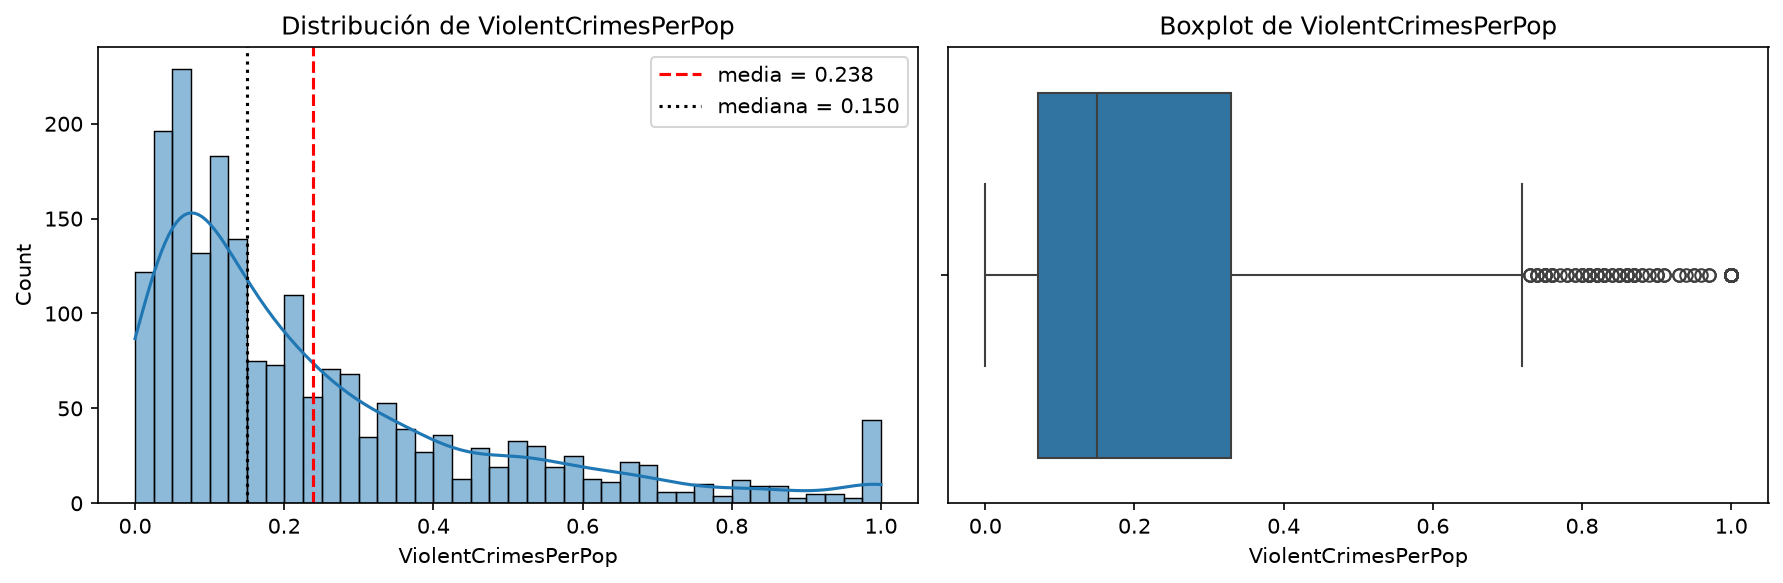
\includegraphics[width=0.9\textwidth]{variable_respuesta.png}
\caption{Distribución de la variable a predecir \texttt{ViolentCrimesPerPop}.}
\end{figure}

La correlación con la respuesta (calculada en el entrenamiento) muestra que la estructura familiar es lo más relacionado con el crimen violento: el porcentaje de hijos nacidos fuera del matrimonio (\texttt{PctIlleg}, $r=0.737$) y el porcentaje de niños que viven con ambos padres (\texttt{PctKids2Par}, $r=-0.736$), seguidos de \texttt{PctFam2Par} ($-0.708$), \texttt{racePctWhite} ($-0.674$), \texttt{PctYoungKids2Par} ($-0.670$) y \texttt{racepctblack} ($0.631$). Después aparecen el ingreso por inversiones (\texttt{pctWInvInc}, $-0.567$), la asistencia pública (\texttt{pctWPubAsst}, $0.565$) y los divorcios. Estas correlaciones coinciden con las que reportan \citet{redmond2002}, pero son asociaciones y no relaciones causales.

\begin{figure}[H]
\centering
\begin{subfigure}{0.45\textwidth}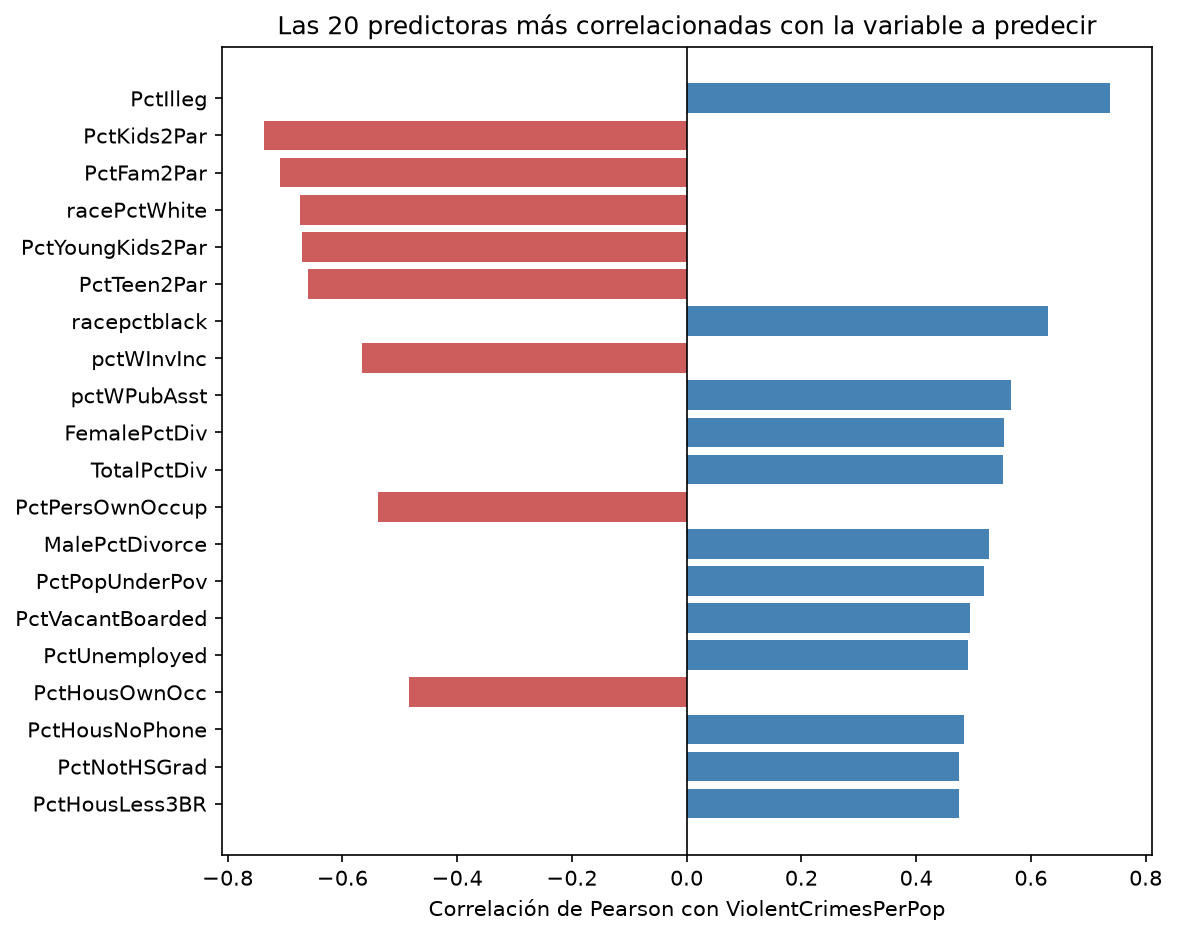
\includegraphics[width=\linewidth]{correlacion_respuesta.png}\caption{Correlación con la respuesta}\end{subfigure}
\begin{subfigure}{0.53\textwidth}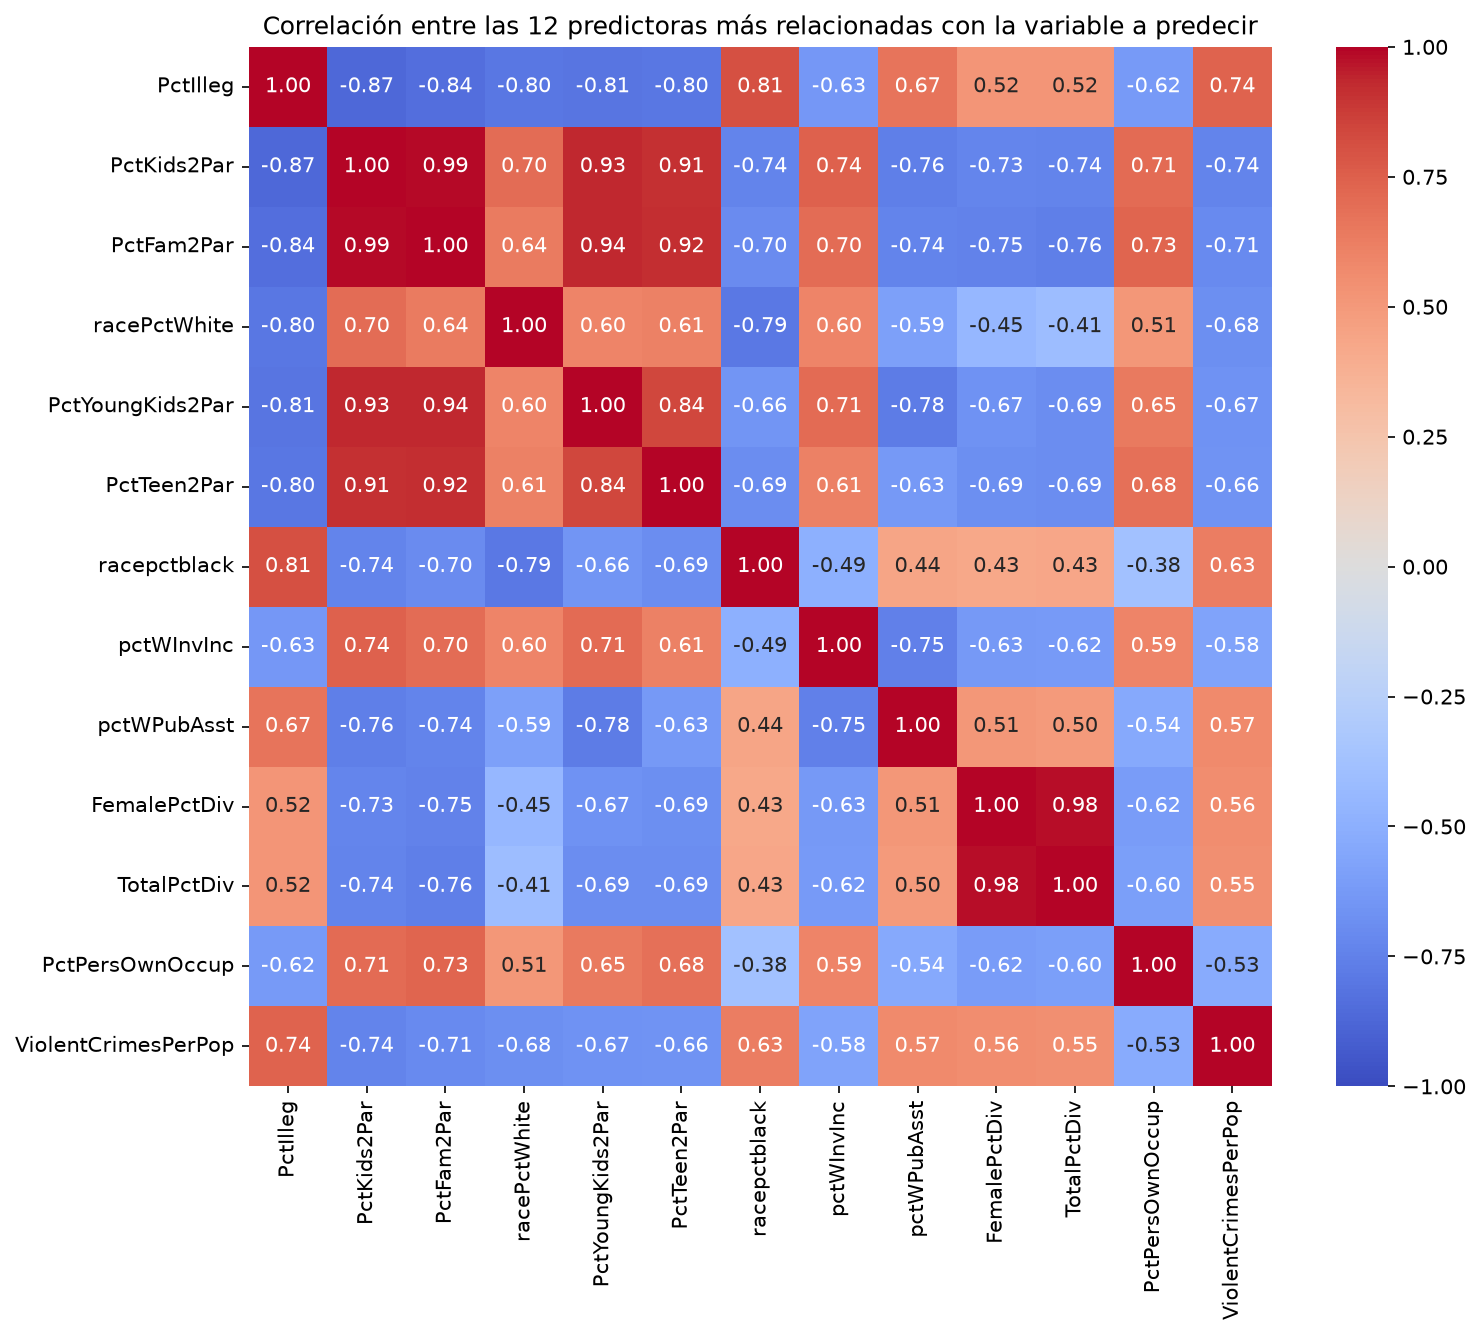
\includegraphics[width=\linewidth]{mapa_calor.png}\caption{Correlación entre las 12 más relacionadas}\end{subfigure}
\caption{Correlaciones de las predictoras con la variable a predecir y entre sí.}
\end{figure}

El mapa de calor muestra el rasgo principal del conjunto: \textbf{una fuerte multicolinealidad}. Hay 49 pares de predictoras con $|r|>0.9$ y 127 con $|r|>0.8$. Muchas variables miden casi lo mismo: \texttt{PctKids2Par}, \texttt{PctFam2Par}, \texttt{PctYoungKids2Par} y \texttt{PctTeen2Par} tienen correlaciones entre 0.9 y 0.99, y lo mismo pasa con las tres variables de divorcio, con los ingresos medianos de hogares y familias, o con los cuartiles del valor de la vivienda. Según \citet{dormann2013}, a partir de $|r|>0.7$ la colinealidad ya distorsiona los coeficientes de un modelo lineal. Por eso esperábamos que MCO tuviera coeficientes inestables y que la regularización ayudara a interpretarlos.

\begin{figure}[H]
\centering
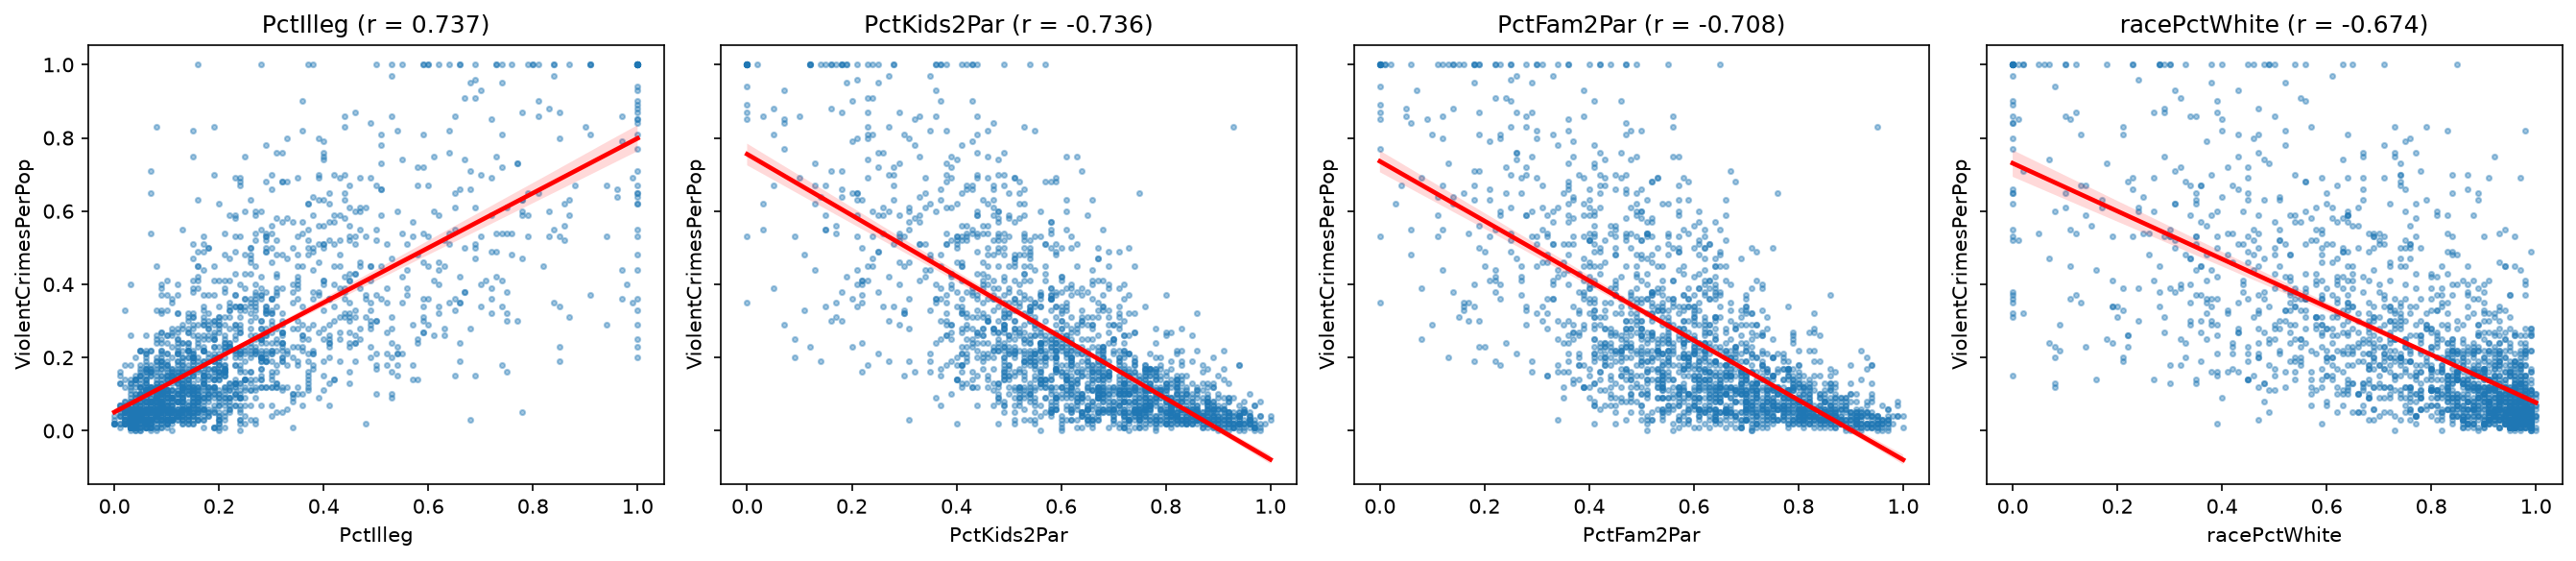
\includegraphics[width=\textwidth]{dispersion_top.png}
\caption{Relación de las cuatro predictoras más correlacionadas con la respuesta, con la recta de mínimos cuadrados.}
\end{figure}

Los diagramas de dispersión muestran relaciones aproximadamente lineales pero con mucha dispersión, que además crece con el valor de la respuesta (heterocedasticidad). La media de la respuesta es 0.244 en el entrenamiento y 0.219 en la prueba, una diferencia normal en una partición aleatoria.

% ======================================================================
\section{Familia 1: modelos lineales}

\subsection{Regresión lineal simple y múltiple}
La regresión simple usa por defecto la predictora más correlacionada con la respuesta en el entrenamiento (\texttt{PctIlleg}), y también probamos la segunda (\texttt{PctKids2Par}), que tiene casi la misma correlación. Las rectas ajustadas son $\hat y = 0.0533 + 0.7523\,\texttt{PctIlleg}$ y $\hat y = 0.7627 - 0.8431\,\texttt{PctKids2Par}$: pasar de una comunidad sin niños con ambos padres a una donde todos los niños viven con ambos padres baja la tasa predicha en 0.84. En la regresión múltiple probamos las 100 predictoras y solo las 50 y 20 más relacionadas con la respuesta (\texttt{SelectKBest} con el estadístico $F$ de la regresión).

\begin{table}[H]
\centering
\small
\caption{Regresión lineal simple y múltiple. En negrita, el mejor modelo de cada algoritmo según el RMSE.}
\begin{tabular}{lcccc}
\toprule
Configuración & RMSE & MAE & ER & $R^2$ \\
\midrule
Lineal simple (\texttt{PctIlleg}) & 0.1490 & 0.1080 & 0.4941 & 0.5433 \\
\textbf{Lineal simple (\texttt{PctKids2Par})} & \textbf{0.1479} & \textbf{0.1067} & \textbf{0.4877} & \textbf{0.5504} \\
\midrule
\textbf{Lineal múltiple (estándar, 100 predictoras)} & \textbf{0.1301} & \textbf{0.0937} & \textbf{0.4284} & \textbf{0.6518} \\
Lineal múltiple (50 atributos) & 0.1314 & 0.0922 & 0.4215 & 0.6449 \\
Lineal múltiple (20 atributos) & 0.1316 & 0.0932 & 0.4263 & 0.6439 \\
\bottomrule
\end{tabular}
\end{table}

\begin{figure}[H]
\centering
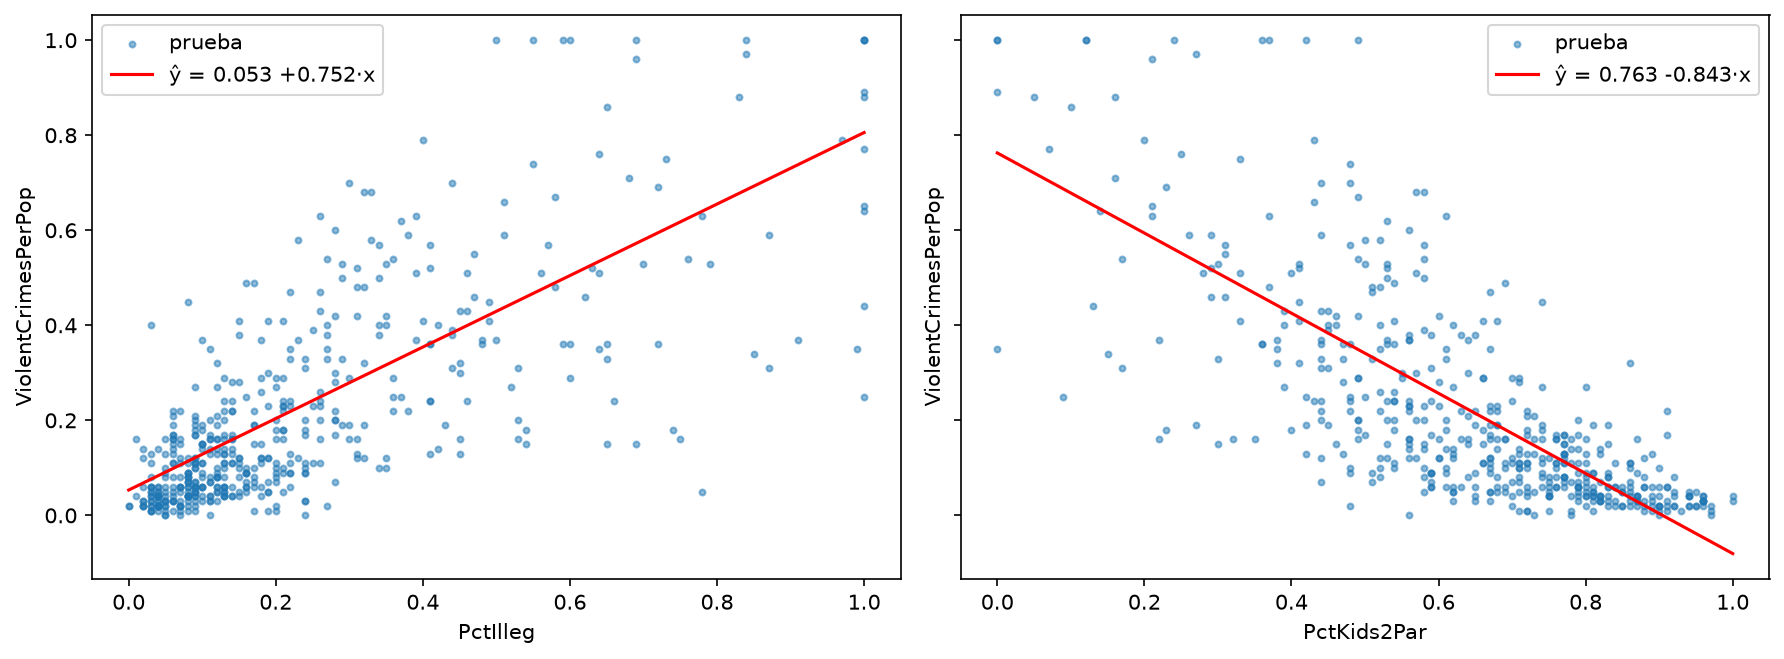
\includegraphics[width=0.85\textwidth]{lineal_simple.png}
\caption{Rectas de la regresión lineal simple sobre el conjunto de prueba.}
\end{figure}

Una sola variable ya explica el 55\,\% de la varianza de la respuesta en la prueba, lo que confirma lo que vimos en el análisis exploratorio. Pasar a las 100 predictoras baja el RMSE de 0.1479 a 0.1301 y sube el $R^2$ a 0.652, es decir, las otras 99 variables solo agregan 10 puntos de $R^2$. Quedarse con 20 o 50 variables casi no cambia el resultado: con 20 el RMSE es 0.1316, y el MAE con 50 incluso es un poco menor. Hay mucha información redundante. Los coeficientes de MCO muestran el problema de la multicolinealidad: los de mayor magnitud son \texttt{TotalPctDiv} ($-0.94$), \texttt{PctPersOwnOccup} ($-0.63$) y \texttt{MalePctDivorce} ($+0.62$). Es decir, el porcentaje total de divorcios tiene un coeficiente negativo enorme mientras que el de hombres divorciados lo tiene positivo, aunque las dos variables tienen correlación positiva con el crimen. Los coeficientes se compensan entre variables casi iguales y no se pueden interpretar uno por uno \citep{dormann2013}. Además, MCO predice tasas negativas para 18 comunidades de prueba, algo imposible.

\subsection{Lasso y LassoCV}
La configuración estándar de scikit-learn (\texttt{alpha}=1) es un buen ejemplo de por qué hay que ajustar este hiperparámetro: con las variables estandarizadas, la penalización es tan fuerte que \textbf{anula los 100 coeficientes} y el modelo predice siempre el promedio del entrenamiento ($R^2=-0.014$). Con $\alpha=0.1$, el valor del código guía, quedan solo 2 variables (\texttt{PctIlleg} y \texttt{PctKids2Par}) y el $R^2$ es 0.399. Con $\alpha=0.01$ quedan 14 variables y el modelo ya es tan bueno como MCO.

\begin{table}[H]
\centering
\small
\caption{Lasso y LassoCV. ``Coef.\ $\neq0$'' es la cantidad de variables que el modelo conserva.}
\begin{tabular}{lccccc}
\toprule
Configuración & Coef.\ $\neq0$ & RMSE & MAE & ER & $R^2$ \\
\midrule
estándar ($\alpha=1$) & 0 & 0.2220 & 0.1770 & 0.8094 & $-0.0136$ \\
$\alpha=0.1$ & 2 & 0.1709 & 0.1330 & 0.6081 & 0.3990 \\
$\alpha=0.01$ & 14 & 0.1297 & 0.0906 & 0.4143 & 0.6538 \\
$\alpha=0.001$ & 52 & 0.1293 & 0.0914 & 0.4181 & 0.6563 \\
\textbf{$\alpha=0.001$, sin escalar} & \textbf{22} & \textbf{0.1290} & \textbf{0.0903} & \textbf{0.4127} & \textbf{0.6578} \\
\midrule
\textbf{LassoCV (10 particiones, $\alpha=0.00066$)} & \textbf{62} & \textbf{0.1297} & \textbf{0.0921} & \textbf{0.4213} & \textbf{0.6539} \\
\bottomrule
\end{tabular}
\end{table}

\begin{figure}[H]
\centering
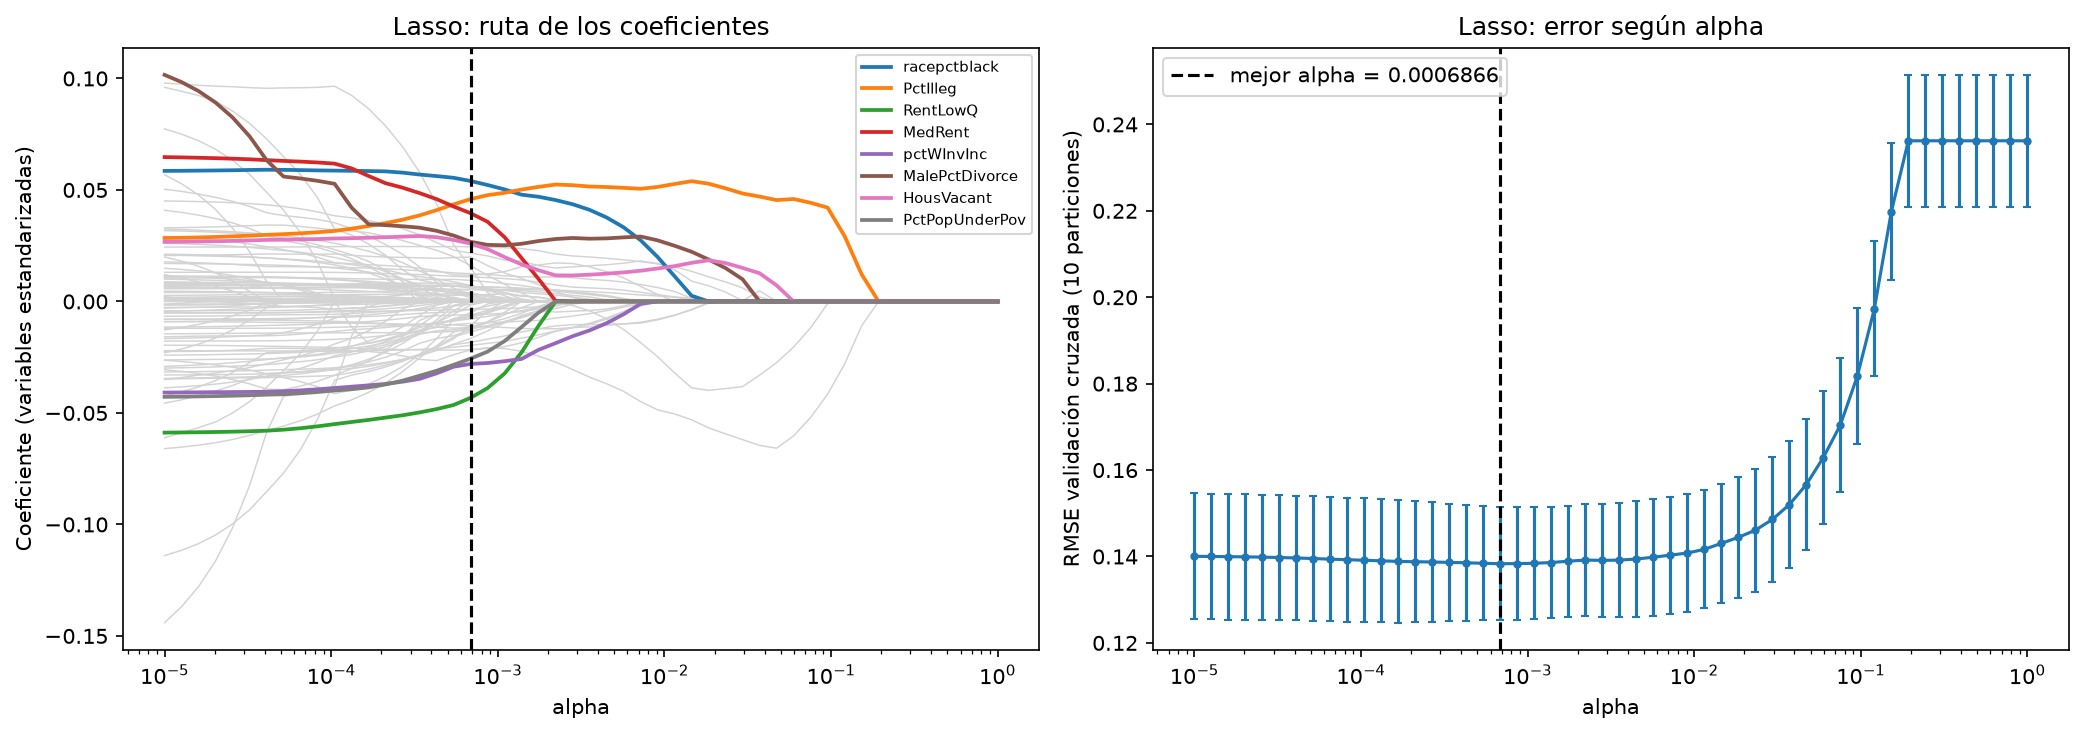
\includegraphics[width=\textwidth]{lasso_ruta.png}
\caption{Lasso: ruta de los coeficientes (en color, las 8 variables de mayor coeficiente en el $\alpha$ óptimo) y RMSE de validación cruzada de 10 particiones según $\alpha$.}
\end{figure}

La ruta de los coeficientes muestra cómo Lasso va eliminando variables al crecer $\alpha$: con $\alpha=10^{-5}$ conserva 98, con $\alpha\approx0.001$ unas 49, con $\alpha=0.01$ solo 14 y a partir de $\alpha\approx0.3$ ninguna. Las dos últimas en salir son \texttt{PctIlleg} y \texttt{PctKids2Par}, las más correlacionadas con la respuesta. El error de validación cruzada es casi plano entre $10^{-5}$ y $10^{-2}$ y crece rápidamente después. \textbf{LassoCV} escogió $\alpha=0.00066$, conserva 62 de las 100 variables y elimina 38, entre ellas muchas de los grupos redundantes: \texttt{racePctWhite} (se queda \texttt{racepctblack}), \texttt{PctFam2Par} y \texttt{PctTeen2Par} (se quedan \texttt{PctKids2Par} y \texttt{PctYoungKids2Par}), \texttt{TotalPctDiv}, \texttt{medIncome}, \texttt{medFamInc} y los tres cuartiles del valor de la vivienda. Es el comportamiento que describen \citet{zou2005}: de cada grupo de variables correlacionadas Lasso conserva una. Sus coeficientes ya tienen signos coherentes: los mayores son \texttt{racepctblack} ($+0.054$), \texttt{PctIlleg} ($+0.046$), \texttt{RentLowQ} ($-0.044$), \texttt{MedRent} ($+0.040$) y \texttt{pctWInvInc} ($-0.028$).

\begin{figure}[H]
\centering
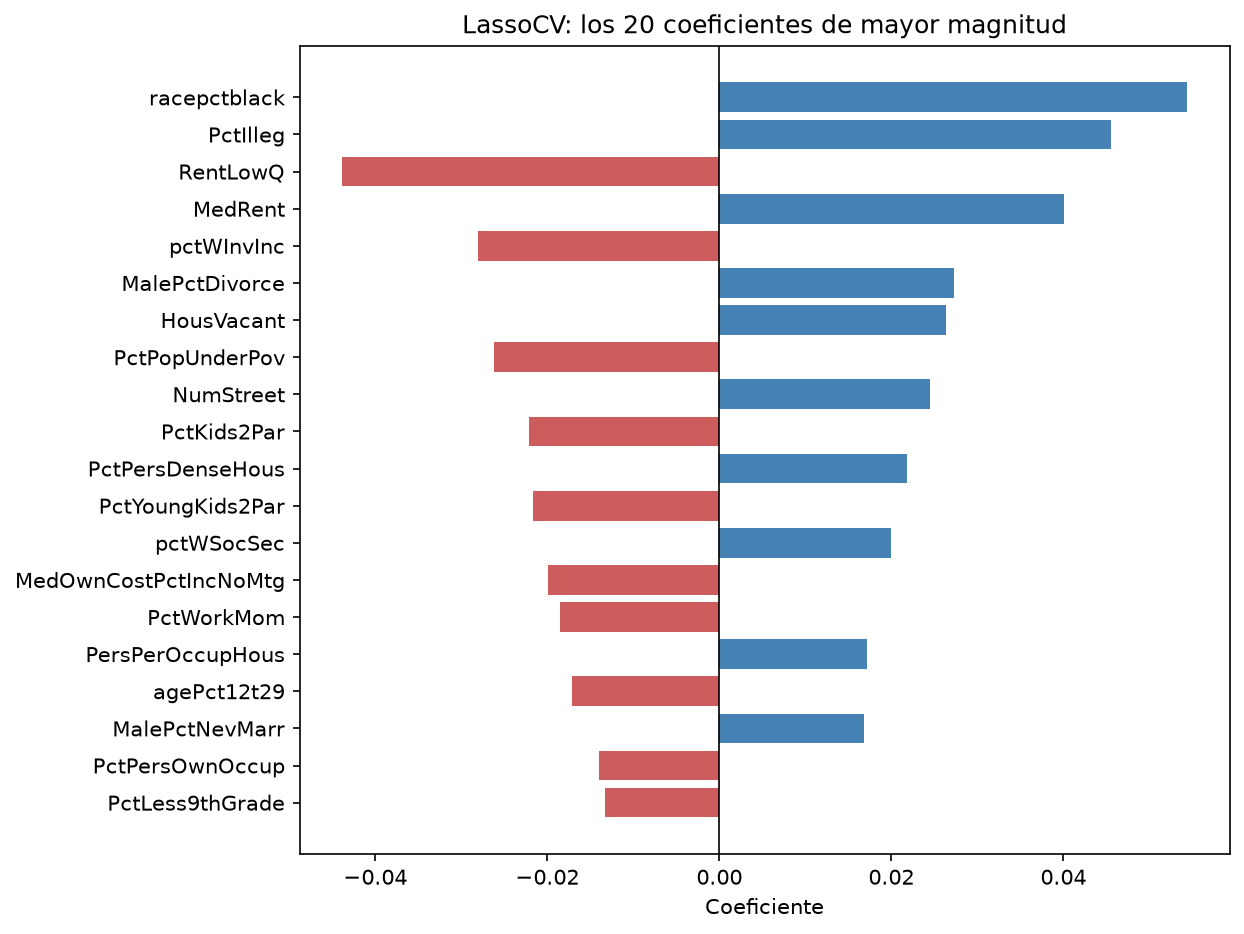
\includegraphics[width=0.7\textwidth]{lassocv_coeficientes.png}
\caption{Los 20 coeficientes de mayor magnitud del modelo LassoCV (variables estandarizadas).}
\end{figure}

El mejor Lasso en la prueba fue el de $\alpha=0.001$ \textbf{sin estandarizar}, con RMSE 0.1290. Como las variables ya están en $[0,1]$ y tienen desviaciones menores a 1, sin estandarizar la misma $\alpha$ penaliza más, y el modelo se queda con solo 22 variables. Que un modelo con 22 variables iguale a MCO con 100 confirma que la mayor parte de la información está concentrada en pocas variables. En la prueba la diferencia con LassoCV es mínima (0.1290 contra 0.1297), y en la validación cruzada repetida (sección~\ref{sec:benchmark}) LassoCV es un poco mejor, así que no hay una ventaja clara de uno sobre el otro.

\subsection{Ridge y RidgeCV}

\begin{table}[H]
\centering
\small
\caption{Ridge y RidgeCV (variables estandarizadas). En negrita, el mejor de cada algoritmo.}
\begin{tabular}{lcccc}
\toprule
Configuración & RMSE & MAE & ER & $R^2$ \\
\midrule
estándar ($\alpha=1$) & 0.1300 & 0.0936 & 0.4280 & 0.6525 \\
$\alpha=10$ & 0.1298 & 0.0932 & 0.4262 & 0.6535 \\
\textbf{$\alpha=100$} & \textbf{0.1290} & \textbf{0.0915} & \textbf{0.4185} & \textbf{0.6578} \\
$\alpha=1000$ & 0.1296 & 0.0913 & 0.4177 & 0.6547 \\
\midrule
RidgeCV (dejando uno fuera, $\alpha=46.4$) & 0.1294 & 0.0923 & 0.4219 & 0.6559 \\
\textbf{RidgeCV (10 particiones, $\alpha=64.3$)} & \textbf{0.1292} & \textbf{0.0920} & \textbf{0.4205} & \textbf{0.6566} \\
\bottomrule
\end{tabular}
\end{table}

\begin{figure}[H]
\centering
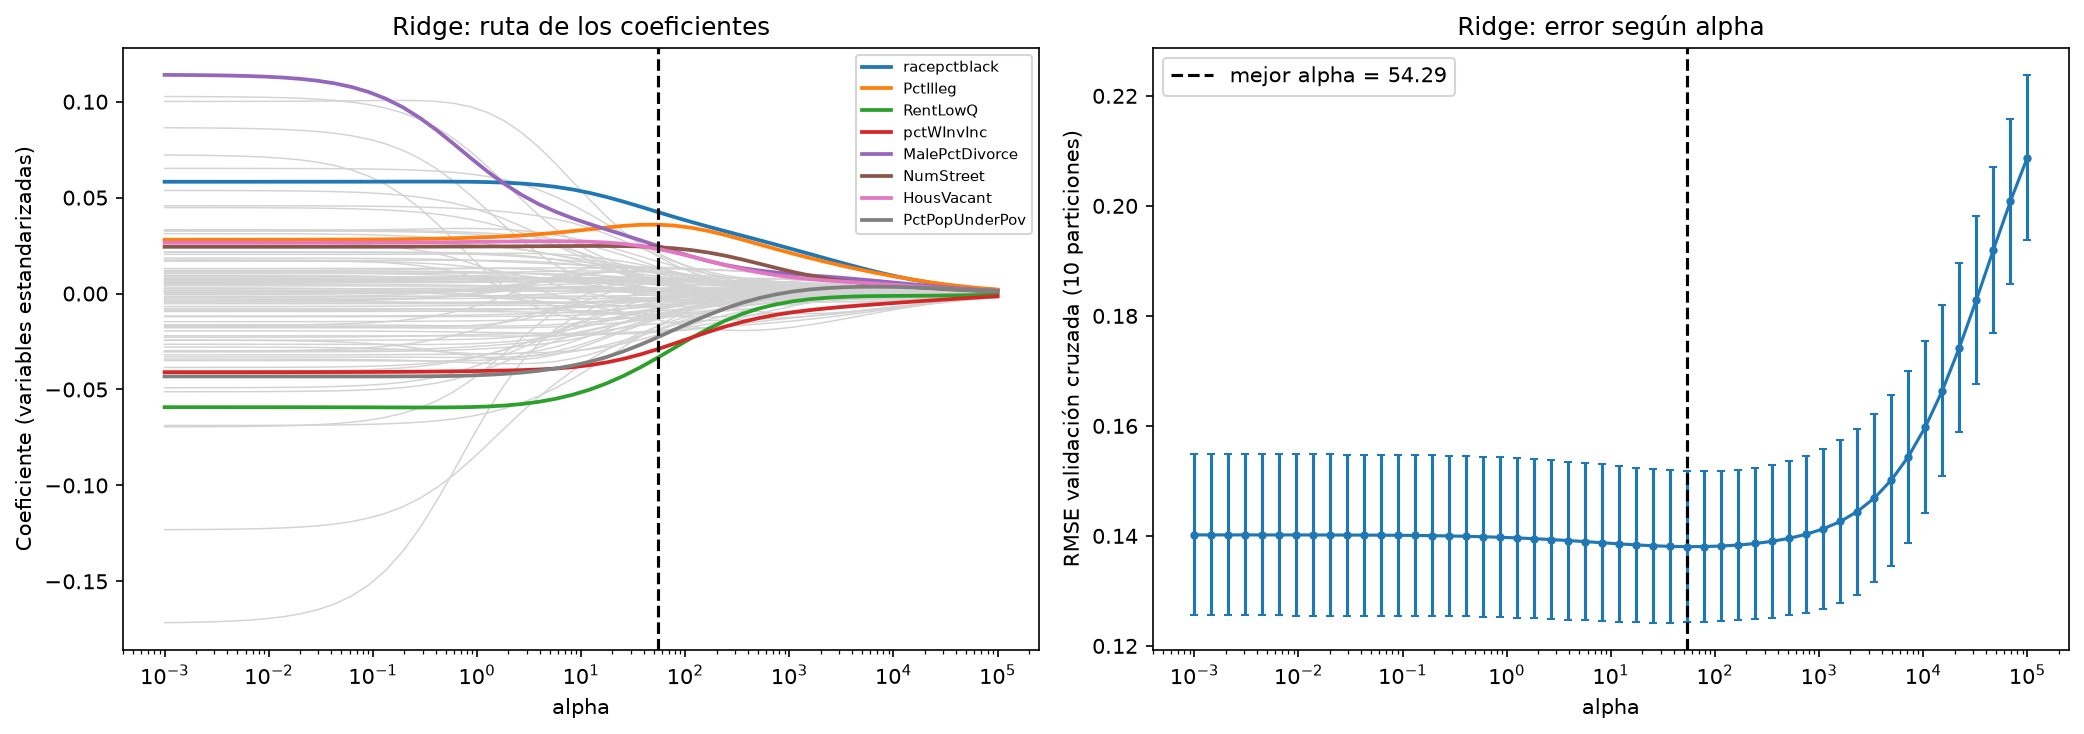
\includegraphics[width=\textwidth]{ridge_ruta.png}
\caption{Ridge: ruta de los coeficientes y RMSE de validación cruzada según $\alpha$.}
\end{figure}

A diferencia de Lasso, la configuración estándar de Ridge ya funciona bien (RMSE 0.1300), porque con $\alpha=1$ y 1495 individuos la penalización es pequeña comparada con la suma de cuadrados. Ridge \textbf{nunca anula coeficientes}: los 100 siguen siendo distintos de cero en toda la ruta, pero se encogen y, sobre todo, dejan de compensarse entre sí. El error de validación cruzada baja levemente hasta $\alpha\approx80$ y sube a partir de $\alpha\approx500$. RidgeCV escogió $\alpha=46.4$ con validación dejando uno fuera y $\alpha=64.3$ con 10 particiones, muy cerca del mejor valor manual ($\alpha=100$, RMSE 0.1290). Con $\alpha=100$ los coeficientes mayores son \texttt{racepctblack} ($+0.038$), \texttt{PctIlleg} ($+0.035$), \texttt{RentLowQ} ($-0.025$) y \texttt{pctWInvInc} ($-0.024$), muy parecidos a los de LassoCV y lejos de los valores de MCO, como describen \citet{hoerl1970}.

\subsection{Comparación dentro de la familia lineal}

\begin{figure}[H]
\centering
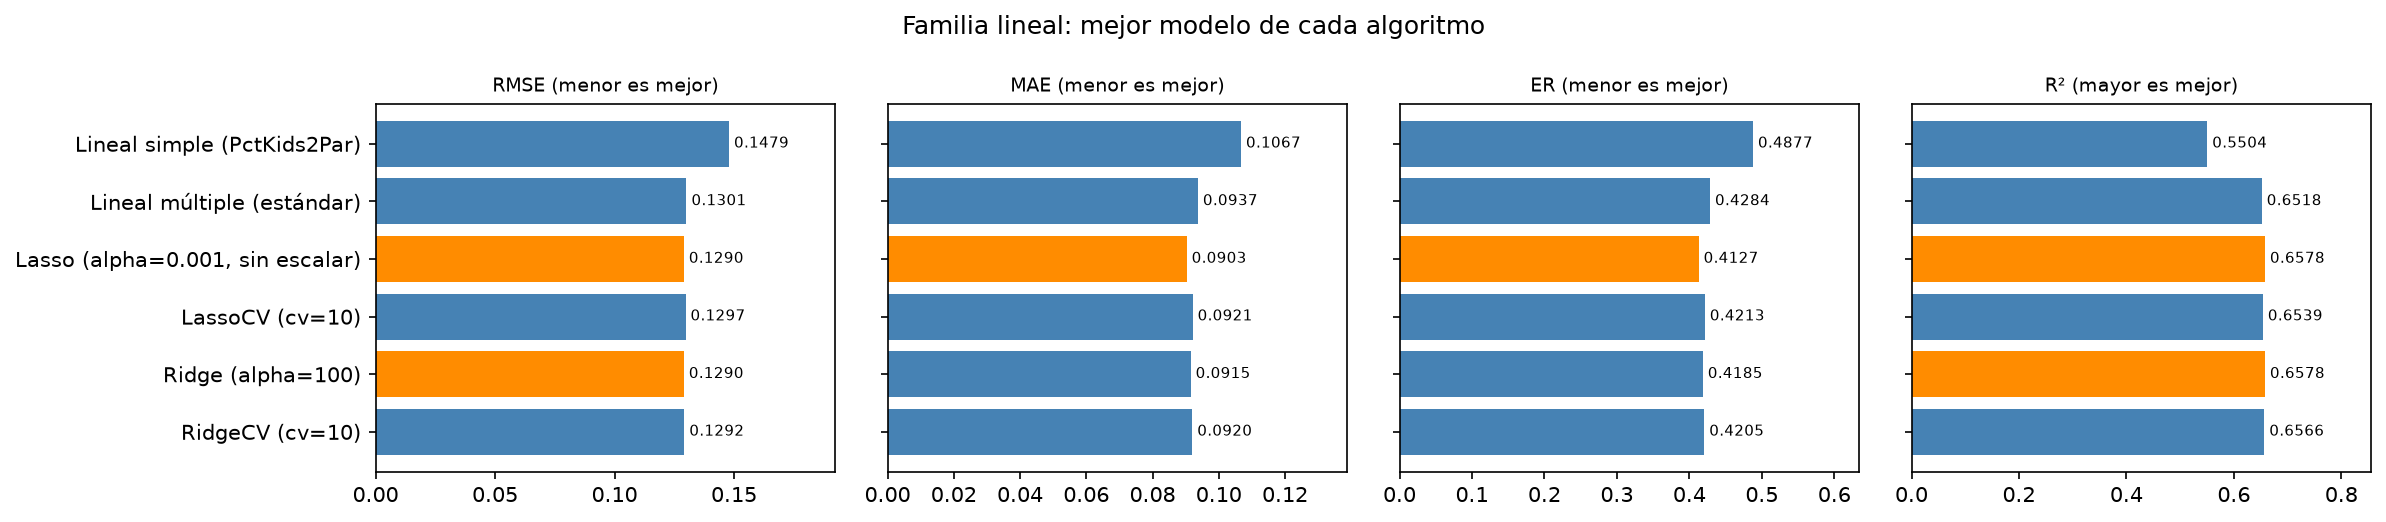
\includegraphics[width=\textwidth]{comparacion_lineal.png}
\caption{Mejor modelo de cada algoritmo de la familia lineal en el conjunto de prueba.}
\end{figure}

Dentro de la familia lineal hay dos grupos claros. La regresión simple queda bastante atrás (RMSE 0.1479, $R^2$ 0.550). Los otros cinco algoritmos quedan prácticamente empatados: Lasso y Ridge con RMSE 0.1290, RidgeCV 0.1292, LassoCV 0.1297 y MCO 0.1301. La regularización mejora el RMSE en menos de 1\,\% respecto a MCO. Esto tiene sentido: con 1495 individuos para 100 coeficientes, la varianza de MCO no es tan grande como para que reducirla cambie mucho la predicción \citep{hastie2009}. La ventaja real de la regularización aquí es otra: produce coeficientes estables e interpretables y, en el caso de Lasso, un modelo con muchas menos variables. Si hubiera que escoger un modelo lineal, escogeríamos \textbf{RidgeCV} o \textbf{LassoCV}: tienen prácticamente el mismo error que los mejores ajustados a mano, pero escogen $\alpha$ solos, sin mirar el conjunto de prueba. Entre los dos, RidgeCV tiene un error un poco menor y LassoCV un modelo más simple.

% ======================================================================
\section{Familia 2: máquinas de vectores de soporte (SVR)}

La configuración estándar de SVR es el kernel rbf con $C=1$, $\varepsilon=0.1$ y $\gamma=$\,\texttt{scale} ($1/(p\cdot\mathrm{Var}(X))=0.01$ con las variables estandarizadas). Para escoger las variaciones del kernel rbf hicimos primero una búsqueda en rejilla con validación cruzada de 5 particiones sobre el entrenamiento, con $C\in\{0.3,1,3,10\}$, $\varepsilon\in\{0.01,0.05,0.1\}$ y $\gamma\in\{0.0005,0.001,0.002,0.005,\texttt{scale}\}$ (60 combinaciones). Las dos mejores fueron $C=1$, $\varepsilon=0.05$, $\gamma=0.002$ (RMSE de validación 0.1367) y $C=3$, $\varepsilon=0.05$, $\gamma=0.001$ (0.1370). También probamos los kernels lineal y polinomial y $C=100$, el valor del código guía.

\begin{table}[H]
\centering
\small
\caption{Configuraciones de SVR. ``VS'' es la cantidad de vectores de soporte (de 1495 individuos de entrenamiento).}
\begin{tabular}{lccccc}
\toprule
Configuración & VS & RMSE & MAE & ER & $R^2$ \\
\midrule
rbf, estándar ($C=1$, $\varepsilon=0.1$) & 583 & 0.1404 & 0.1024 & 0.4685 & 0.5944 \\
rbf, $C=100$ & 630 & 0.1465 & 0.1072 & 0.4902 & 0.5583 \\
rbf, $\varepsilon=0.01$ & 1353 & 0.1354 & 0.0938 & 0.4290 & 0.6228 \\
\textbf{rbf, $C=1$, $\varepsilon=0.05$, $\gamma=0.002$} & \textbf{830} & \textbf{0.1267} & \textbf{0.0853} & \textbf{0.3902} & \textbf{0.6696} \\
rbf, $C=3$, $\varepsilon=0.05$, $\gamma=0.001$ & 844 & 0.1273 & 0.0854 & 0.3907 & 0.6665 \\
lineal, estándar & 541 & 0.1341 & 0.0957 & 0.4378 & 0.6301 \\
lineal, $C=0.01$, $\varepsilon=0.01$ & 1351 & 0.1280 & 0.0871 & 0.3982 & 0.6631 \\
polinomial, estándar (grado 3) & 644 & 0.1600 & 0.1113 & 0.5090 & 0.4732 \\
polinomial, grado 2, $C=0.1$, $\varepsilon=0.01$ & 1383 & 0.1546 & 0.1086 & 0.4966 & 0.5086 \\
\bottomrule
\end{tabular}
\end{table}

\begin{figure}[H]
\centering
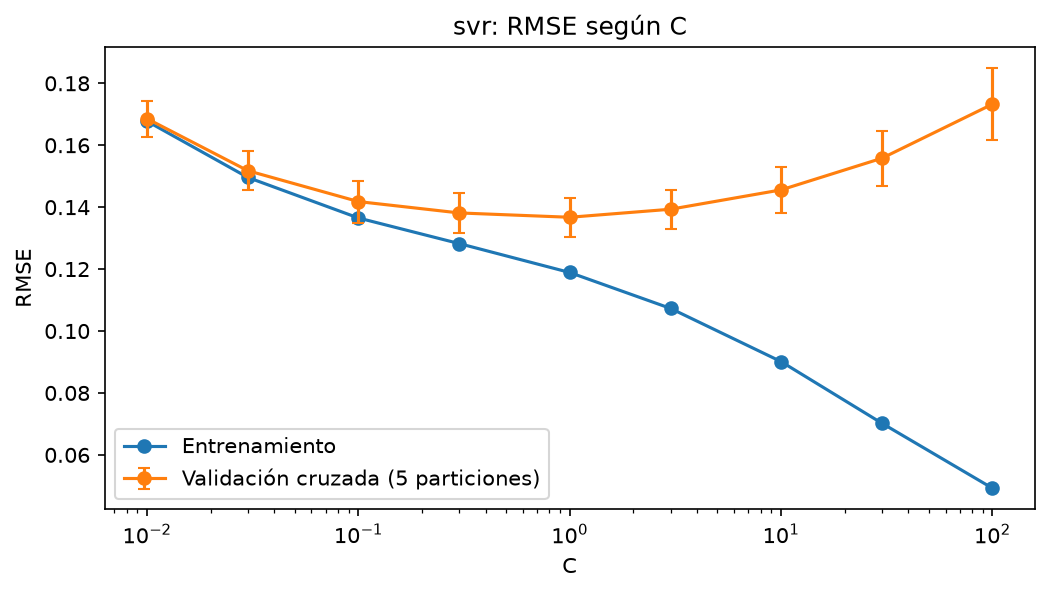
\includegraphics[width=0.75\textwidth]{svr_curva_C.png}
\caption{SVR rbf ($\gamma=0.002$, $\varepsilon=0.05$): RMSE de entrenamiento y de validación cruzada según $C$.}
\end{figure}

El SVR estándar es peor que la regresión lineal múltiple (RMSE 0.1404 contra 0.1301). La razón principal es $\varepsilon$: un tubo de ancho 0.1 es casi la mitad de la desviación estándar de la respuesta (0.233), así que el modelo ignora todos los errores menores que 0.1 y en una variable donde la mitad de los valores son menores que 0.15 eso es demasiado tolerante. Solo con bajar $\varepsilon$ a 0.01 el RMSE baja a 0.1354. El segundo factor es $\gamma$: con $\gamma=0.01$ el kernel es muy local para 100 dimensiones, y bajarlo a 0.002 da una función más suave. El \textbf{mejor SVR} ($C=1$, $\varepsilon=0.05$, $\gamma=0.002$) tiene RMSE 0.1267, MAE 0.0853 y $R^2$ 0.670, \textbf{el mejor resultado de todo el laboratorio en la prueba}. La curva de $C$ muestra el equilibrio entre sesgo y varianza \citep{smola2004}: con $C=0.01$ el modelo es casi constante (RMSE de validación 0.169), el mínimo está en $C=1$ (0.137) y a partir de ahí el error de entrenamiento sigue bajando mientras el de validación sube, hasta 0.173 con $C=100$. Por eso el $C=100$ del código guía empeora el modelo.

Entre kernels, el lineal bien ajustado ($C=0.01$, RMSE 0.1280) queda muy cerca del rbf y supera a todos los modelos lineales de mínimos cuadrados, porque la pérdida $\varepsilon$-insensible es lineal en los errores grandes y es menos sensible a las comunidades atípicas que los mínimos cuadrados \citep{smola2004}. El polinomial es el peor (RMSE 0.1546 en el mejor caso): las interacciones de grado 2 o 3 entre 100 variables crean demasiados términos y el modelo sobreajusta. Que el rbf suave le gane al lineal por poco indica que la relación es \textbf{casi lineal}, con no linealidades leves.

\begin{figure}[H]
\centering
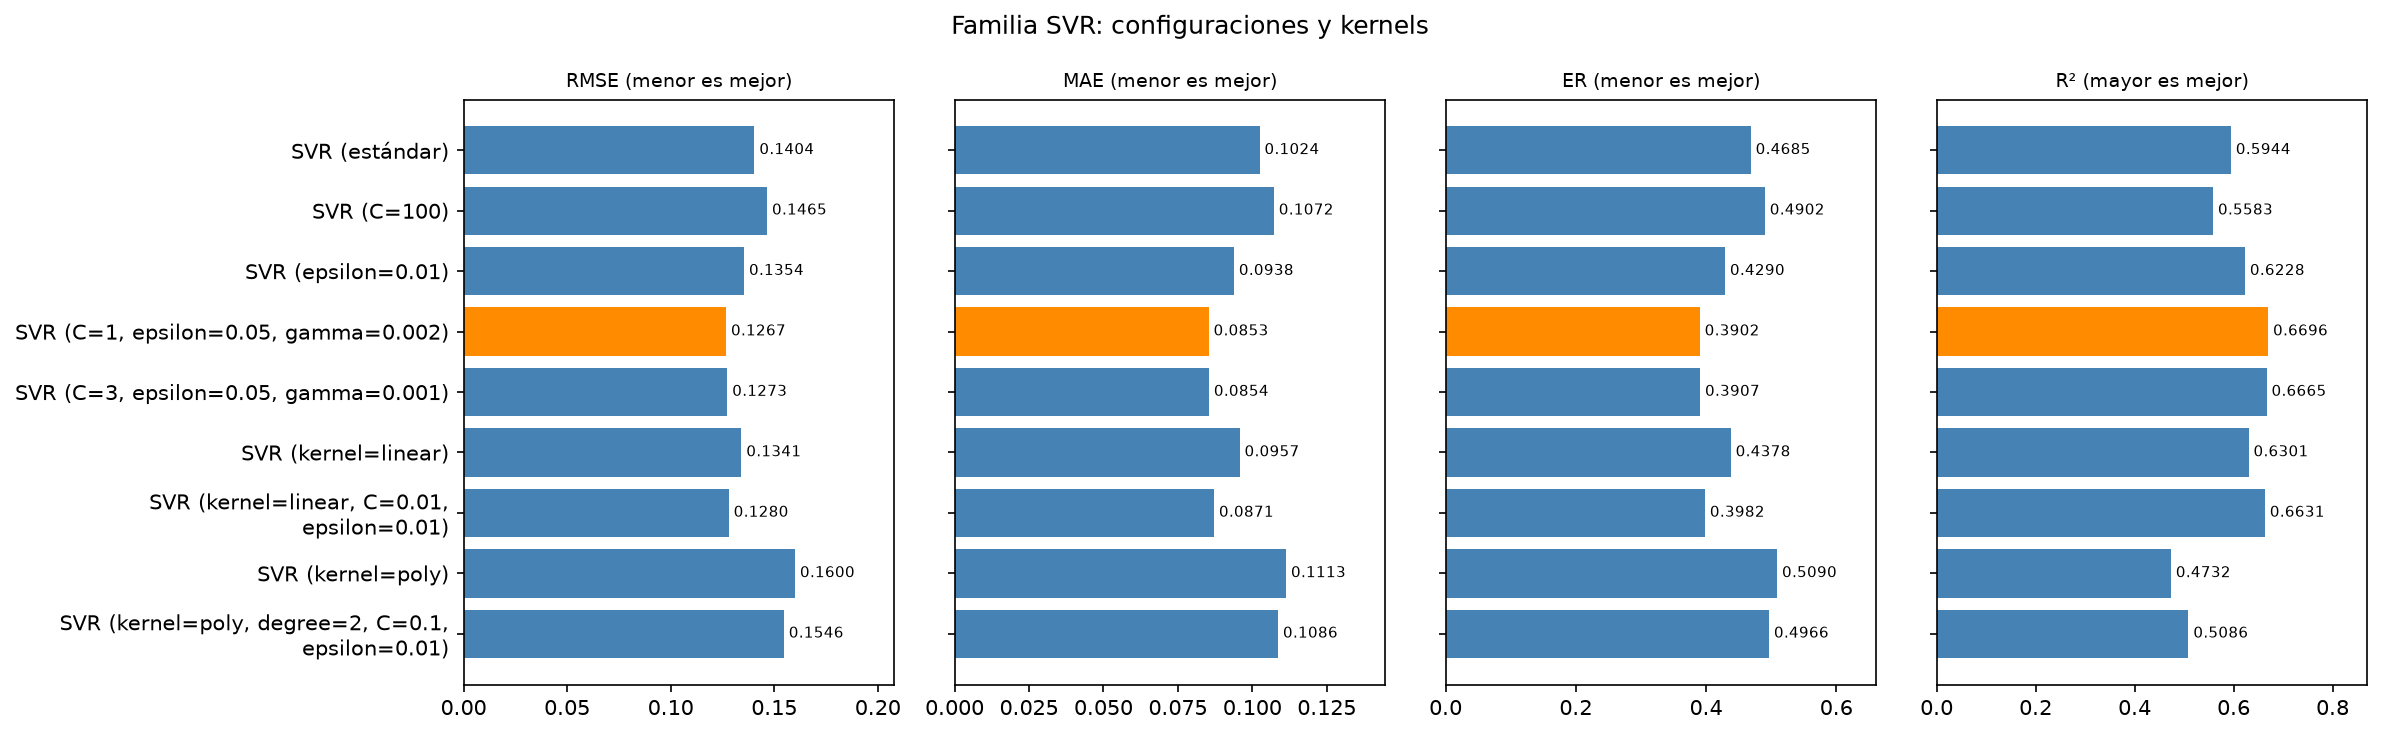
\includegraphics[width=\textwidth]{comparacion_svr.png}
\caption{Comparación de las configuraciones y kernels de SVR en el conjunto de prueba.}
\end{figure}

% ======================================================================
\section{Familia 3: árboles de decisión y ensambles}

\subsection{Árbol de decisión}

\begin{table}[H]
\centering
\small
\caption{Configuraciones del árbol de regresión.}
\begin{tabular}{lcccc}
\toprule
Configuración & RMSE & MAE & ER & $R^2$ \\
\midrule
estándar (sin límite) & 0.1841 & 0.1233 & 0.5641 & 0.3031 \\
\texttt{max\_depth}=3 & 0.1468 & 0.1015 & 0.4642 & 0.5569 \\
\texttt{max\_depth}=4 & 0.1486 & 0.1009 & 0.4612 & 0.5456 \\
\textbf{\texttt{max\_depth}=5, \texttt{min\_samples\_leaf}=20} & \textbf{0.1460} & \textbf{0.1002} & \textbf{0.4581} & \textbf{0.5614} \\
\texttt{min\_samples\_leaf}=30 & 0.1473 & 0.1018 & 0.4657 & 0.5538 \\
\texttt{ccp\_alpha}=0.0005 & 0.1465 & 0.1027 & 0.4696 & 0.5586 \\
\bottomrule
\end{tabular}
\end{table}

\begin{figure}[H]
\centering
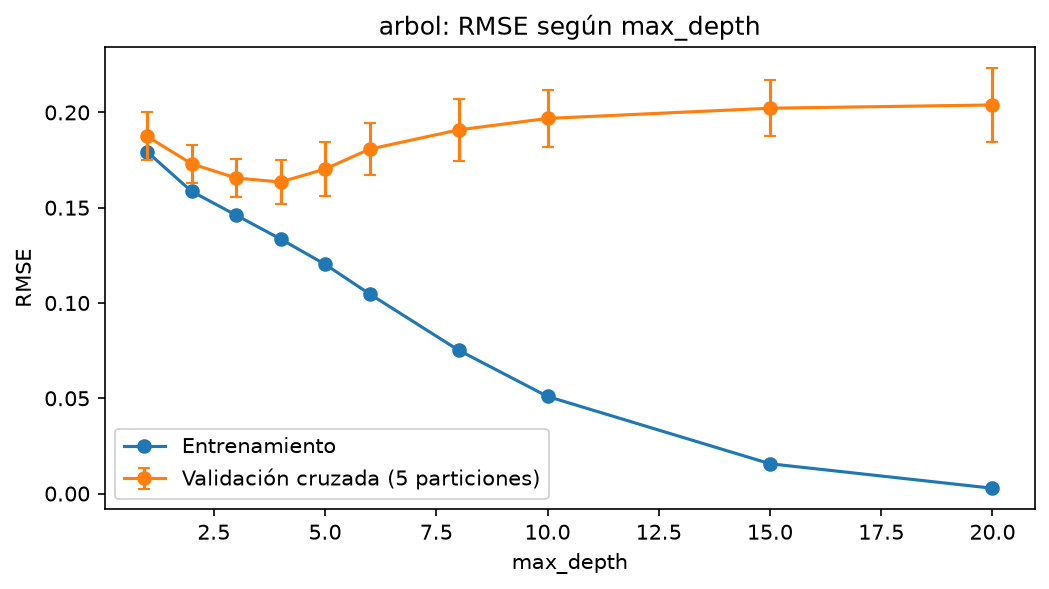
\includegraphics[width=0.75\textwidth]{dt_curva_profundidad.png}
\caption{Árbol de regresión: RMSE de entrenamiento y de validación cruzada según la profundidad máxima.}
\end{figure}

El árbol estándar creció hasta 24 niveles y 1143 hojas, casi una hoja por cada individuo de entrenamiento: memorizó los datos y tiene el $R^2$ más bajo de los modelos razonables (0.303). La curva de profundidad lo muestra con claridad: el error de entrenamiento cae a casi cero, pero el de validación es mínimo con profundidad 4 (0.164) y después sube hasta 0.204 \citep{breiman1984}. Cualquier forma de limitar el árbol (profundidad, hojas mínimas o poda) da resultados parecidos, con RMSE entre 0.146 y 0.149. El \textbf{mejor árbol} (profundidad 5 y al menos 20 individuos por hoja, 26 hojas) tiene RMSE 0.1460, un poco mejor que la regresión simple pero lejos de los demás modelos.

\begin{figure}[H]
\centering
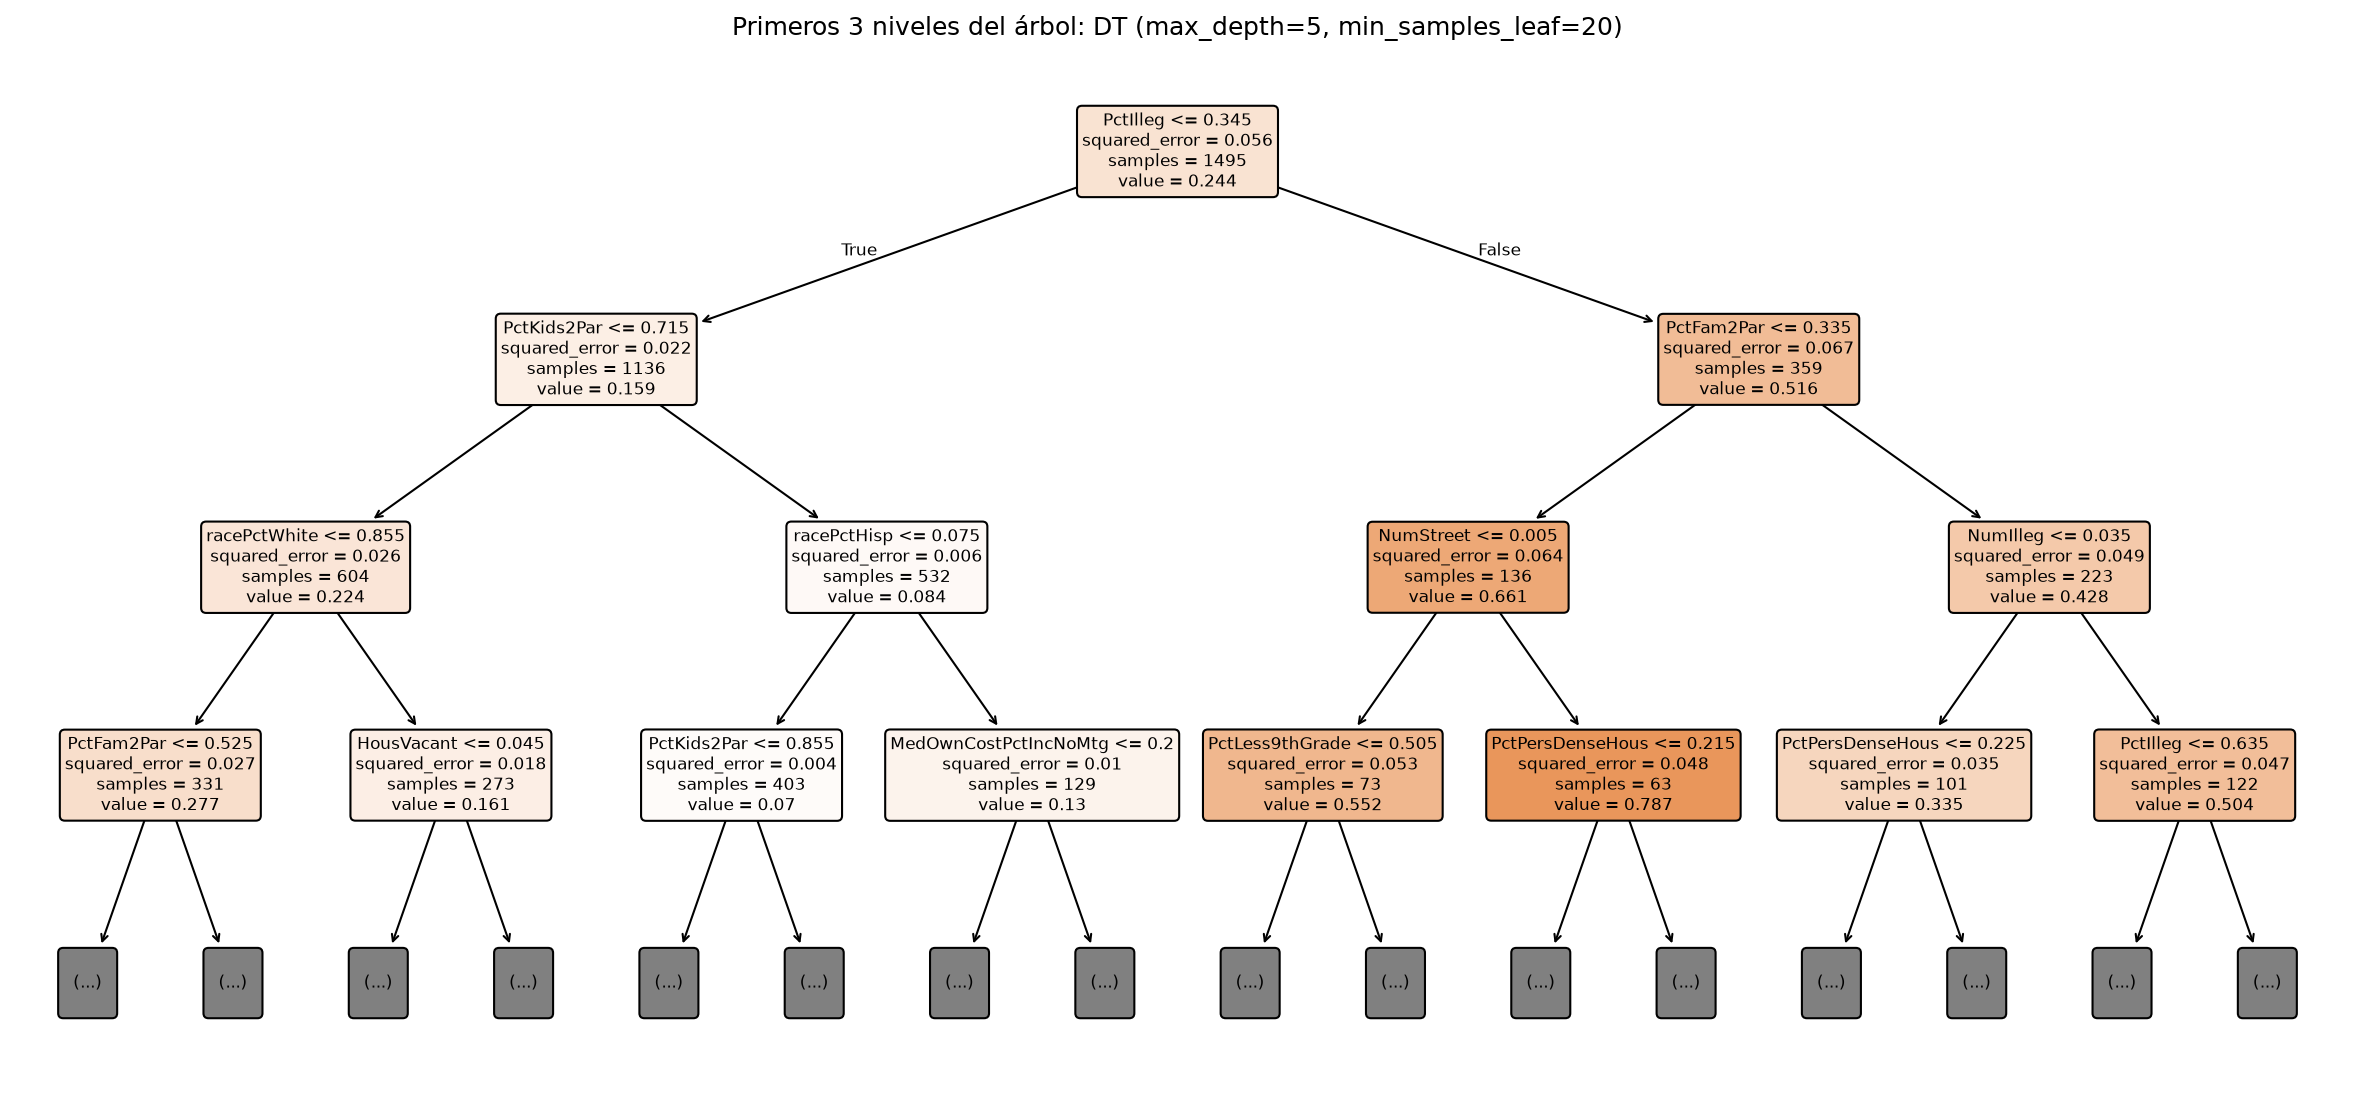
\includegraphics[width=\textwidth]{dt_arbol.png}
\caption{Primeros tres niveles del mejor árbol de regresión.}
\end{figure}

El árbol es fácil de leer. La primera división es \texttt{PctIlleg}~$\le0.345$: las 1136 comunidades que la cumplen tienen una tasa promedio de 0.159, y las 359 restantes de 0.516. En la rama de baja tasa, la siguiente pregunta es si \texttt{PctKids2Par}~$>0.715$ (promedio 0.084); en la de alta, si \texttt{PctFam2Par}~$\le0.335$ (promedio 0.661), y entre esas, las que tienen personas en la calle (\texttt{NumStreet}) y viviendas muy densas llegan a 0.787. Las mismas variables de estructura familiar del análisis exploratorio aparecen arriba del árbol. El problema es que la predicción es escalonada: 26 valores posibles para una respuesta continua, lo que explica su error más alto.

\subsection{Random Forest}

\begin{table}[H]
\centering
\small
\caption{Configuraciones de Random Forest.}
\begin{tabular}{lcccc}
\toprule
Configuración & RMSE & MAE & ER & $R^2$ \\
\midrule
estándar (100 árboles, todas las variables) & 0.1314 & 0.0921 & 0.4214 & 0.6451 \\
\texttt{max\_depth}=2 (código guía) & 0.1436 & 0.1036 & 0.4738 & 0.5759 \\
500 árboles & 0.1317 & 0.0918 & 0.4198 & 0.6435 \\
500 árboles, \texttt{max\_features}=0.33 & 0.1300 & 0.0910 & 0.4162 & 0.6522 \\
\textbf{500 árboles, \texttt{max\_features}=0.33, \texttt{min\_samples\_leaf}=5} & \textbf{0.1292} & \textbf{0.0887} & \textbf{0.4058} & \textbf{0.6568} \\
\bottomrule
\end{tabular}
\end{table}

El bosque estándar ya baja el RMSE de 0.184 (un árbol sin límite) a 0.131: promediar 100 árboles elimina casi toda la varianza de un árbol individual \citep{breiman2001}. Pasar de 100 a 500 árboles no cambia nada, porque el error ya se estabilizó. Lo que sí ayuda es usar $p/3$ variables por división, como recomienda \citet{breiman2001} para regresión: con variables tan redundantes, si cada árbol puede usar siempre \texttt{PctIlleg} o \texttt{PctKids2Par}, todos los árboles se parecen; obligarlos a usar otras los hace más distintos y el promedio mejora \citep{probst2019}. El \textbf{mejor bosque} agrega hojas de al menos 5 individuos (RMSE 0.1292, $R^2$ 0.657). Limitar los árboles a profundidad 2, como en el código guía, los vuelve demasiado simples (RMSE 0.1436).

\subsection{XGBoost}

\begin{table}[H]
\centering
\small
\caption{Configuraciones de XGBoost.}
\begin{tabular}{>{\raggedright\arraybackslash}p{8cm}cccc}
\toprule
Configuración & RMSE & MAE & ER & $R^2$ \\
\midrule
estándar (100 árboles, tasa 0.3, profundidad 6) & 0.1379 & 0.0935 & 0.4275 & 0.6087 \\
300 árboles, tasa 0.05, profundidad 3 & 0.1331 & 0.0884 & 0.4042 & 0.6359 \\
\textbf{500 árboles, tasa 0.02, profundidad 3, \texttt{subsample}=0.8, \texttt{colsample\_bytree}=0.5} & \textbf{0.1291} & \textbf{0.0866} & \textbf{0.3961} & \textbf{0.6574} \\
500 árboles, tasa 0.02, profundidad 2, \texttt{subsample}=0.8, \texttt{colsample\_bytree}=0.5, \texttt{min\_child\_weight}=5 & 0.1297 & 0.0880 & 0.4026 & 0.6540 \\
\bottomrule
\end{tabular}
\end{table}

Como en el Laboratorio 02, XGBoost estándar sobreajusta (tasa 0.3 y árboles de profundidad 6 para solo 1495 individuos). Con una tasa más baja, árboles poco profundos y submuestreo de filas y columnas, el RMSE baja de 0.1379 a 0.1291 \citep{friedman2001,chen2016}. El submuestreo de columnas cumple la misma función que \texttt{max\_features} en Random Forest.

\begin{figure}[H]
\centering
\begin{subfigure}{0.49\textwidth}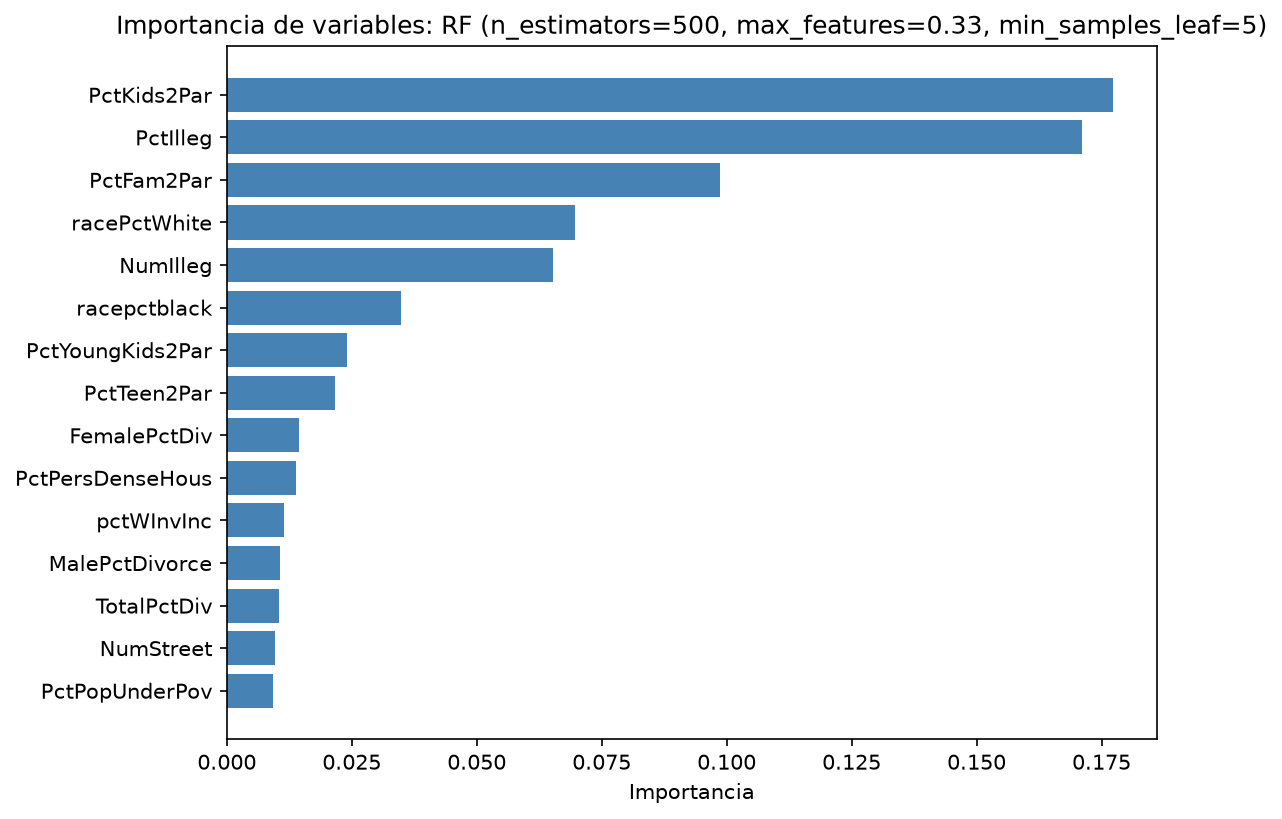
\includegraphics[width=\linewidth]{rf_importancia.png}\caption{Random Forest}\end{subfigure}
\begin{subfigure}{0.49\textwidth}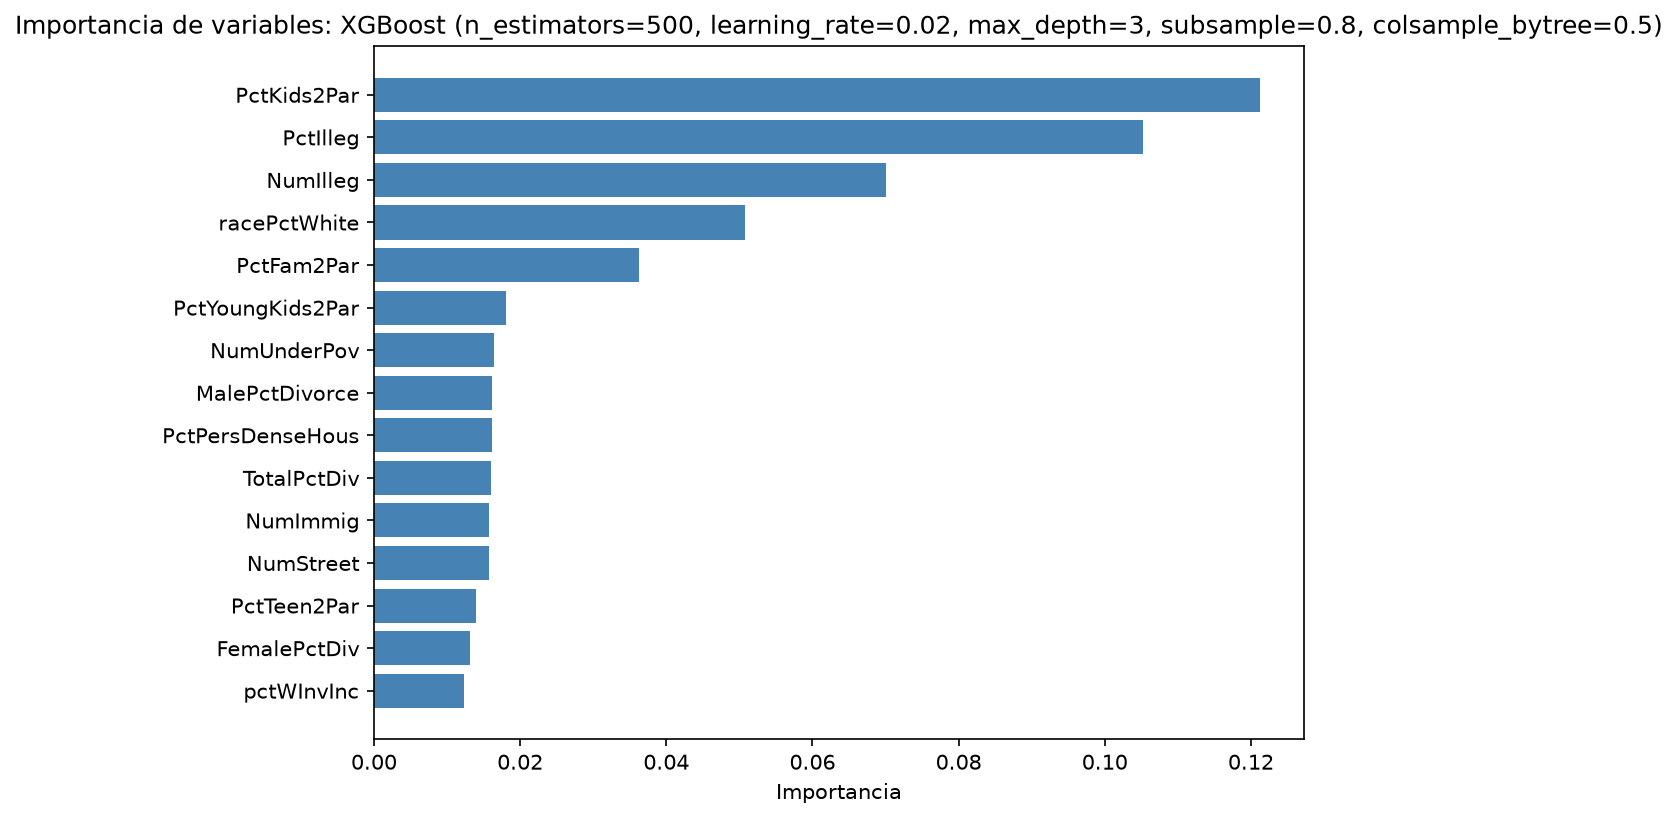
\includegraphics[width=\linewidth]{xgboost_importancia.png}\caption{XGBoost}\end{subfigure}
\caption{Importancia de las 15 variables más importantes en los mejores modelos de ensamble.}
\end{figure}

La importancia de variables coincide con todo lo anterior. En el árbol, \texttt{PctIlleg} concentra el 61.5\,\% de la importancia. En los ensambles, gracias al muestreo de variables, la importancia se reparte más: en Random Forest \texttt{PctKids2Par} (17.7\,\%), \texttt{PctIlleg} (17.1\,\%), \texttt{PctFam2Par} (9.9\,\%), \texttt{racePctWhite} (7.0\,\%) y \texttt{NumIlleg} (6.5\,\%), y en XGBoost las mismas en un orden parecido. Un detalle importante es que la importancia se reparte entre variables equivalentes: \texttt{PctKids2Par}, \texttt{PctFam2Par}, \texttt{PctYoungKids2Par} y \texttt{PctTeen2Par} miden casi lo mismo, así que la importancia de cada una por separado subestima la de la estructura familiar en conjunto.

\subsection{Comparación dentro de la familia de árboles}

\begin{figure}[H]
\centering
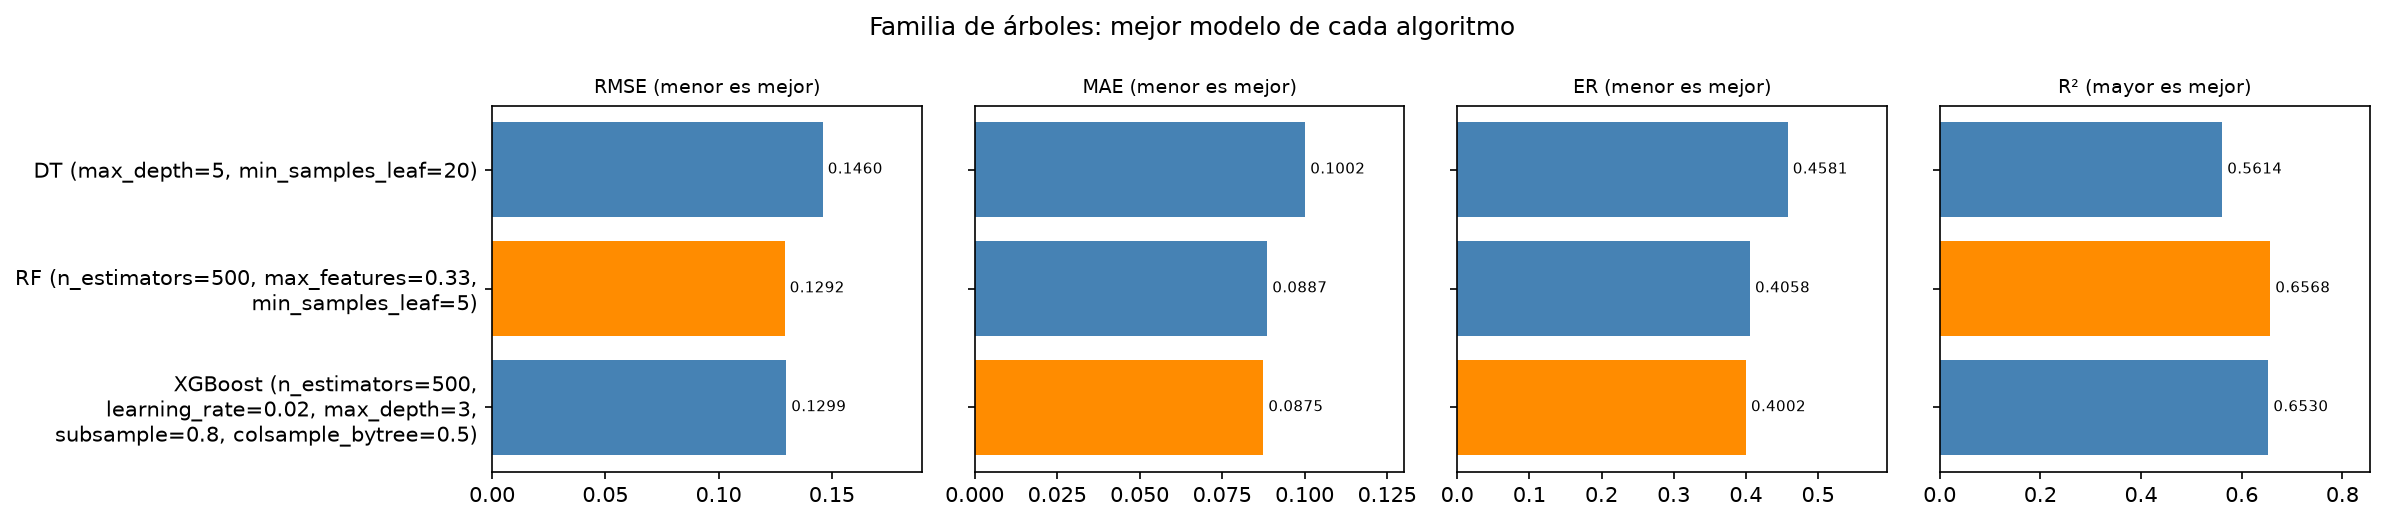
\includegraphics[width=\textwidth]{comparacion_arboles.png}
\caption{Mejor modelo de cada algoritmo de la familia de árboles en el conjunto de prueba.}
\end{figure}

Dentro de esta familia la diferencia entre un árbol y un ensamble es grande: el RMSE baja de 0.1460 a 0.1292 (RF) y 0.1291 (XGBoost), y el $R^2$ sube de 0.561 a 0.657. RF y XGBoost quedan empatados en RMSE, pero XGBoost tiene menor MAE (0.0866 contra 0.0887), o sea, se equivoca menos en la comunidad típica. El árbol solo vale la pena por su interpretabilidad.

% ======================================================================
\section{Comparación entre familias y benchmarking}
\label{sec:benchmark}

\subsection{Comparación en el conjunto de prueba}

\begin{table}[H]
\centering
\small
\caption{Mejor modelo de cada algoritmo en el conjunto de prueba, ordenados por RMSE.}
\begin{tabular}{>{\raggedright\arraybackslash}p{6.6cm}lcccc}
\toprule
Modelo & Familia & RMSE & MAE & ER & $R^2$ \\
\midrule
\textbf{SVR (rbf, $C=1$, $\varepsilon=0.05$, $\gamma=0.002$)} & \textbf{Núcleos} & \textbf{0.1267} & \textbf{0.0853} & \textbf{0.3902} & \textbf{0.6696} \\
Lasso ($\alpha=0.001$, sin escalar) & Lineal & 0.1290 & 0.0903 & 0.4127 & 0.6578 \\
Ridge ($\alpha=100$) & Lineal & 0.1290 & 0.0915 & 0.4185 & 0.6578 \\
XGBoost (500 árboles, tasa 0.02, prof.\ 3) & Árboles & 0.1291 & 0.0866 & 0.3961 & 0.6574 \\
RidgeCV (10 particiones) & Lineal & 0.1292 & 0.0920 & 0.4205 & 0.6566 \\
RF (500 árboles, $p/3$, hoja mín.\ 5) & Árboles & 0.1292 & 0.0887 & 0.4058 & 0.6568 \\
LassoCV (10 particiones) & Lineal & 0.1297 & 0.0921 & 0.4213 & 0.6539 \\
Lineal múltiple (estándar) & Lineal & 0.1301 & 0.0937 & 0.4284 & 0.6518 \\
DT (prof.\ 5, hoja mín.\ 20) & Árboles & 0.1460 & 0.1002 & 0.4581 & 0.5614 \\
Lineal simple (\texttt{PctKids2Par}) & Lineal & 0.1479 & 0.1067 & 0.4877 & 0.5504 \\
\bottomrule
\end{tabular}
\end{table}

\begin{figure}[H]
\centering
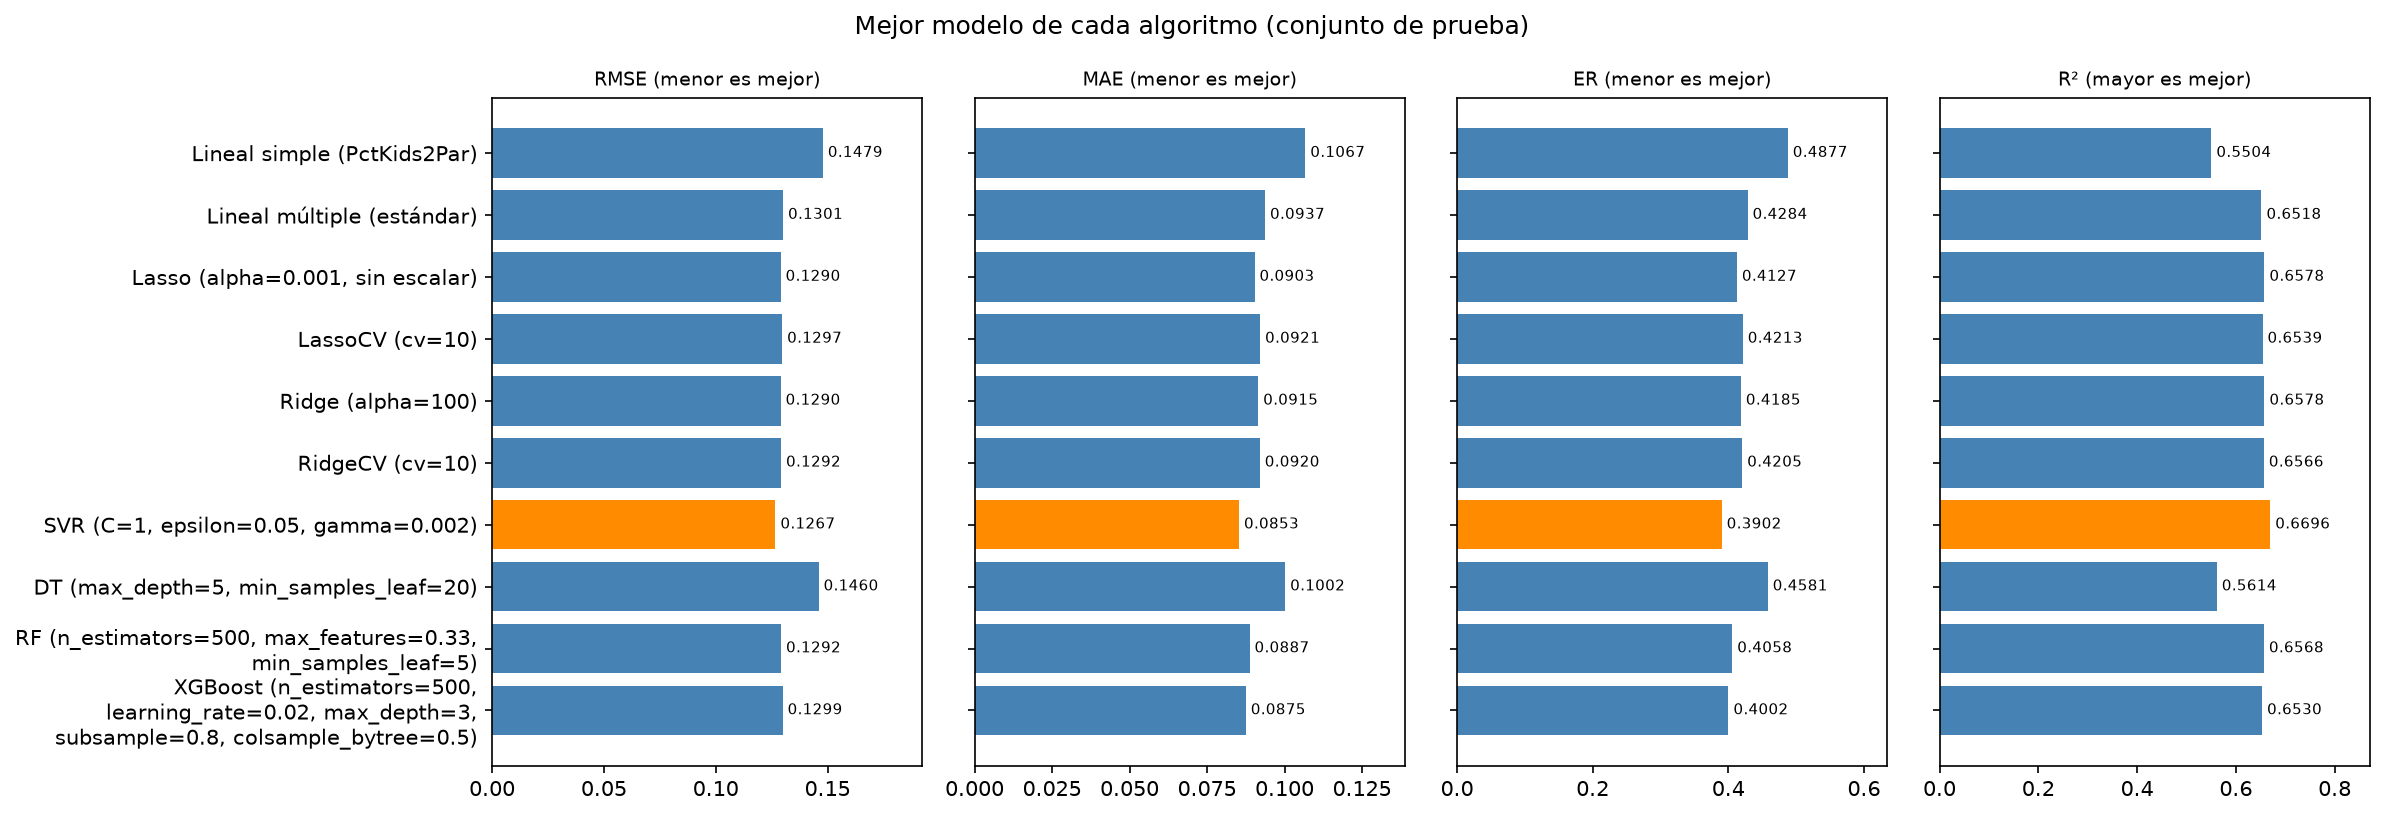
\includegraphics[width=\textwidth]{comparacion_mejores.png}
\caption{Índices del mejor modelo de cada algoritmo en el conjunto de prueba (en naranja, el mejor en cada índice).}
\end{figure}

En la prueba, el SVR rbf es el mejor en los cuatro índices. Le siguen, prácticamente empatados (RMSE entre 0.1290 y 0.1301), los ensambles de árboles y los modelos lineales regularizados, y muy atrás el árbol individual y la regresión simple. Entre familias, el mejor de cada una es: \textbf{núcleos} SVR rbf (0.1267), \textbf{lineal} Lasso o Ridge (0.1290) y \textbf{árboles} XGBoost (0.1291). Se nota una diferencia entre los índices: los modelos lineales igualan a los ensambles en RMSE, pero tienen un MAE claramente mayor (0.090--0.094 contra 0.087--0.089). Los mínimos cuadrados se ajustan para no cometer errores grandes y a cambio se equivocan un poco más en las comunidades típicas, mientras que SVR y los árboles son más robustos a las comunidades atípicas \citep{willmott2005}.

\begin{figure}[H]
\centering
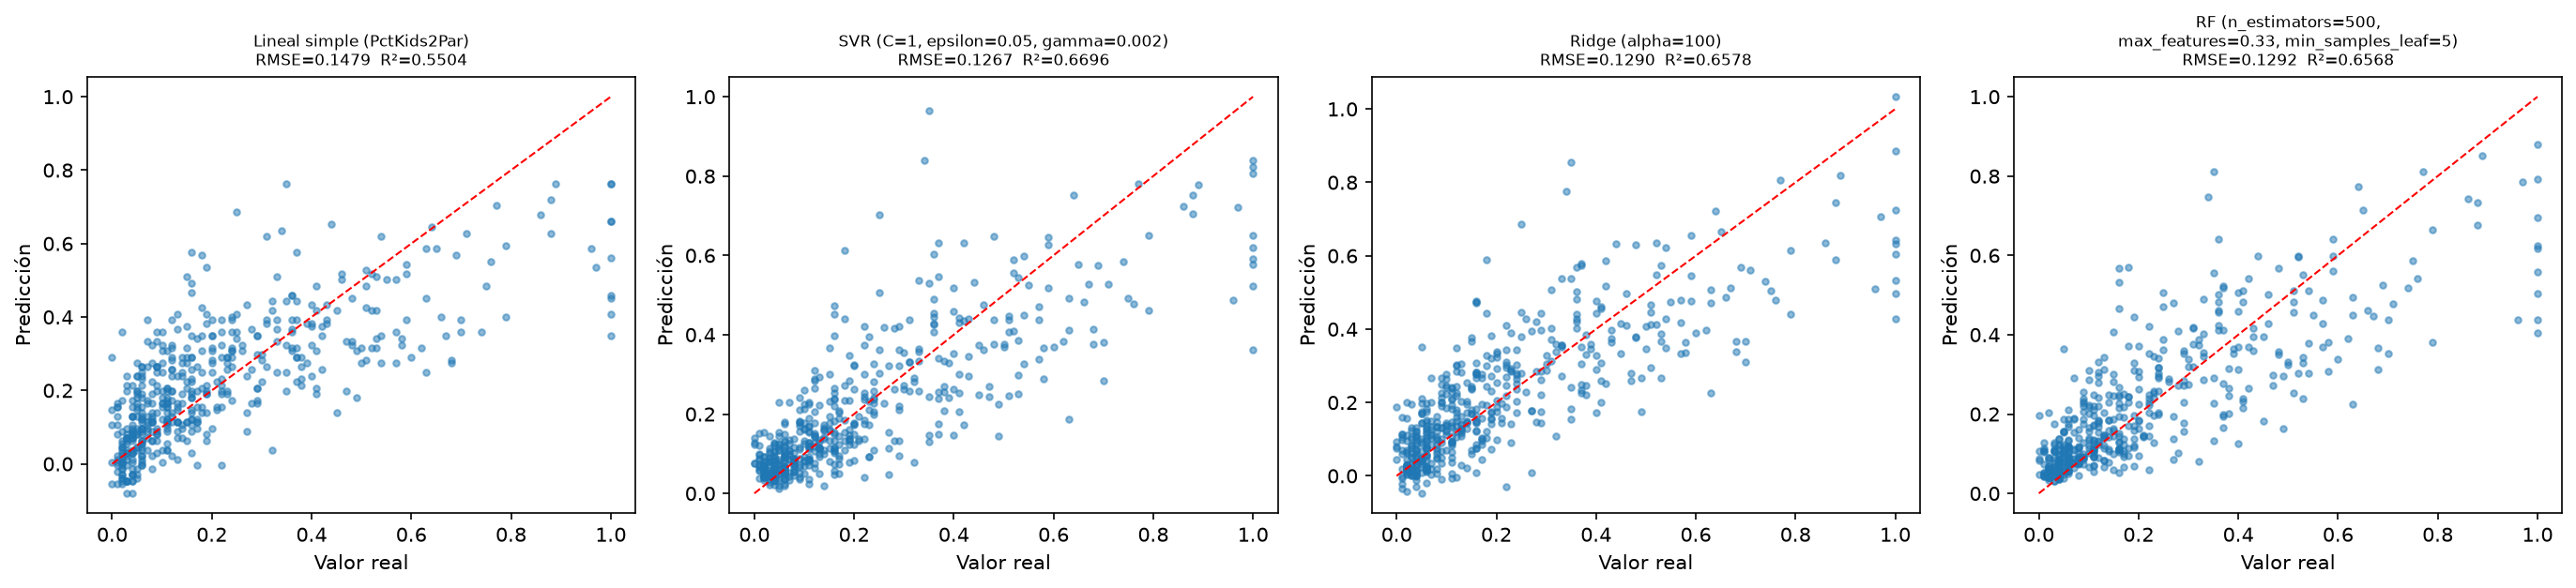
\includegraphics[width=\textwidth]{real_vs_predicho.png}
\caption{Valores reales contra predicciones en el conjunto de prueba: regresión simple y mejor modelo de cada familia.}
\end{figure}

Los gráficos de valores reales contra predicciones muestran que todos los modelos tienen el mismo patrón: aciertan bastante en las comunidades con poco crimen, pero \textbf{subestiman} las de mucho crimen. Las 9 comunidades de prueba con valor real 1 reciben predicciones entre 0.35 y 0.76 con la regresión simple y entre 0.36 y 0.84 con el SVR. Los modelos lineales además predicen tasas negativas, que son imposibles: 34 comunidades con la regresión simple, 18 con MCO y 14 con Ridge. Esto no pasó con el SVR rbf ni con los ensambles; en Random Forest no puede pasar, porque sus predicciones son promedios de valores observados.

\begin{figure}[H]
\centering
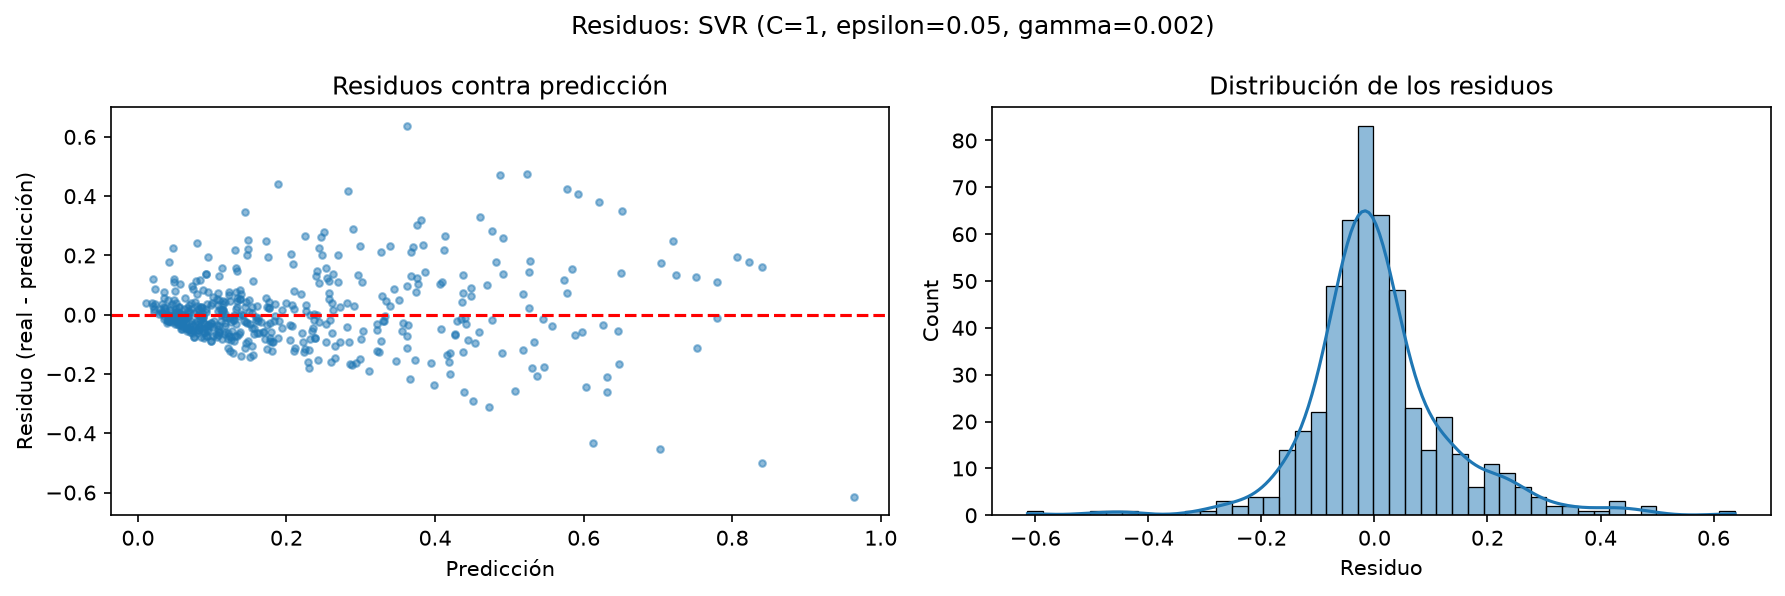
\includegraphics[width=\textwidth]{residuos.png}
\caption{Residuos del mejor modelo (SVR rbf) en el conjunto de prueba.}
\end{figure}

Los residuos del mejor modelo confirman ese patrón. Están centrados en cero y su distribución es simétrica en el centro, pero su dispersión crece con la predicción (heterocedasticidad) y la cola derecha es más larga. En las 59 comunidades de prueba con un valor real mayor a 0.5, el residuo promedio es $+0.189$: el modelo las subestima sistemáticamente. En las 185 con valor real menor a 0.1, el residuo promedio es $-0.035$. Esto es la regresión hacia la media: con un $R^2$ de 0.67, el modelo no tiene suficiente información para distinguir las comunidades extremas, y les asigna valores más cercanos al promedio \citep{james2013}. Mejorar esto probablemente requiere información que no está en las predictoras, no un algoritmo distinto.

\subsection{Benchmarking con validación cruzada repetida}
El conjunto de prueba tiene solo 499 comunidades, y las diferencias entre los ocho mejores modelos son de milésimas de RMSE. Para saber si son reales, evaluamos el mejor modelo de cada algoritmo con validación cruzada de 10 particiones repetida 3 veces sobre el entrenamiento (30 particiones iguales para todos) \citep{hothorn2005,kohavi1995}.

\begin{table}[H]
\centering
\small
\caption{Benchmarking: promedio y desviación estándar en las 30 particiones (validación cruzada $10\times3$). El rango promedio es la posición media del modelo en cada partición (1 = el mejor).}
\setlength{\tabcolsep}{4pt}
\begin{tabular}{>{\raggedright\arraybackslash}p{5.6cm}lcccc}
\toprule
Modelo & Familia & RMSE & MAE & $R^2$ & Rango \\
\midrule
\textbf{SVR (rbf, $C=1$, $\varepsilon=0.05$, $\gamma=0.002$)} & \textbf{Núcleos} & \textbf{0.1345 $\pm$ 0.0146} & \textbf{0.0906} & \textbf{0.671 $\pm$ 0.054} & \textbf{2.33} \\
XGBoost (500 árboles, tasa 0.02, prof.\ 3) & Árboles & 0.1365 $\pm$ 0.0136 & 0.0932 & 0.661 $\pm$ 0.057 & 3.50 \\
RF (500 árboles, $p/3$, hoja mín.\ 5) & Árboles & 0.1371 $\pm$ 0.0136 & 0.0946 & 0.658 $\pm$ 0.057 & 3.53 \\
Ridge ($\alpha=100$) & Lineal & 0.1384 $\pm$ 0.0129 & 0.0970 & 0.652 $\pm$ 0.056 & 4.40 \\
RidgeCV (10 particiones) & Lineal & 0.1384 $\pm$ 0.0129 & 0.0971 & 0.651 $\pm$ 0.057 & 4.43 \\
LassoCV (10 particiones) & Lineal & 0.1390 $\pm$ 0.0127 & 0.0976 & 0.648 $\pm$ 0.056 & 5.27 \\
Lasso ($\alpha=0.001$, sin escalar) & Lineal & 0.1400 $\pm$ 0.0127 & 0.0975 & 0.643 $\pm$ 0.055 & 6.17 \\
Lineal múltiple (estándar) & Lineal & 0.1403 $\pm$ 0.0135 & 0.1001 & 0.641 $\pm$ 0.060 & 6.60 \\
DT (prof.\ 5, hoja mín.\ 20) & Árboles & 0.1583 $\pm$ 0.0140 & 0.1077 & 0.543 $\pm$ 0.081 & 9.20 \\
Lineal simple (\texttt{PctKids2Par}) & Lineal & 0.1599 $\pm$ 0.0114 & 0.1171 & 0.535 $\pm$ 0.057 & 9.57 \\
\bottomrule
\end{tabular}
\end{table}

\begin{figure}[H]
\centering
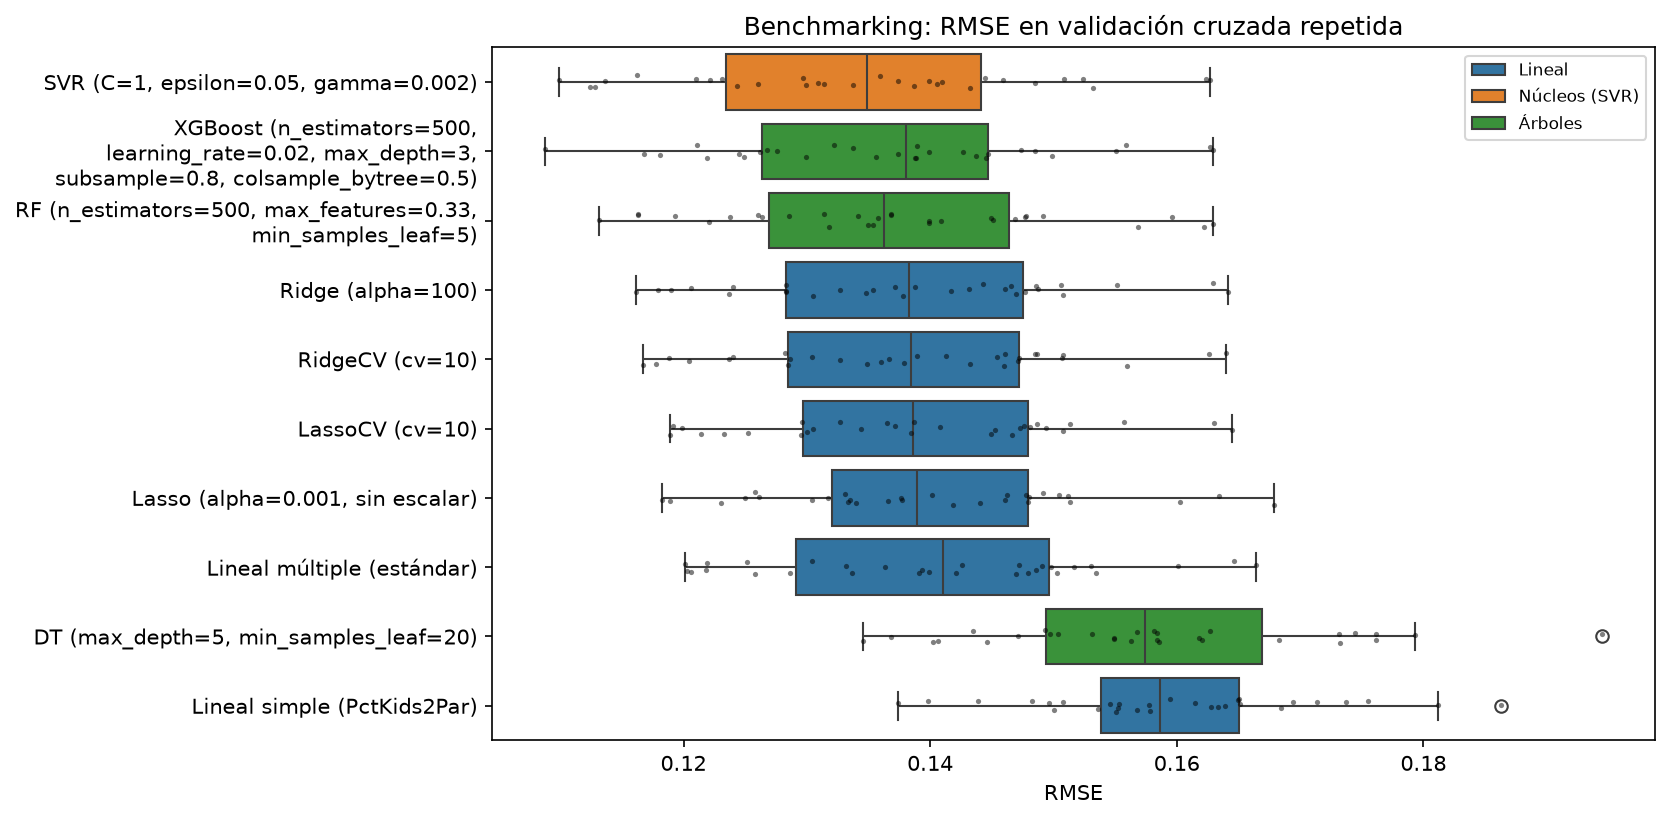
\includegraphics[width=\textwidth]{benchmark_rmse.png}
\caption{Distribución del RMSE de cada modelo en las 30 particiones de la validación cruzada repetida, coloreado por familia.}
\end{figure}

La validación cruzada separa a los modelos mejor que el conjunto de prueba. El orden queda: \textbf{SVR rbf}, luego los dos \textbf{ensambles de árboles}, luego los \textbf{lineales regularizados}, MCO, y al final el árbol individual y la regresión simple. SVR tiene el menor RMSE promedio (0.1345) y el mejor rango promedio (2.33): es el mejor modelo en la mayoría de las particiones. A diferencia de la prueba, aquí los modelos lineales sí quedan claramente por debajo de los ensambles, y dentro de ellos se ve el orden que esperábamos por la teoría: Ridge y RidgeCV (0.1384) son mejores que LassoCV (0.1390), el Lasso de 22 variables (0.1400) y MCO (0.1403). La desviación estándar entre particiones (0.013--0.015) es mucho mayor que las diferencias entre los mejores modelos, pero como las particiones son las mismas para todos, lo que importa es si un modelo le gana al otro de forma consistente partición por partición, y eso es lo que miden las pruebas estadísticas \citep{demsar2006}.

\begin{table}[H]
\centering
\small
\caption{Pruebas estadísticas sobre el RMSE de las 30 particiones. Friedman: $\chi^2=170.8$ con 9 grados de libertad, $p=4.3\times10^{-32}$. Wilcoxon: SVR rbf contra cada modelo, con valores $p$ corregidos por Holm.}
\begin{tabular}{lccc}
\toprule
SVR rbf contra & Diferencia de RMSE & $p$ Holm & ¿Significativa ($\alpha=0.05$)? \\
\midrule
XGBoost & 0.0020 & 0.058 & no \\
Random Forest & 0.0026 & 0.017 & sí \\
RidgeCV & 0.0039 & $7.3\times10^{-5}$ & sí \\
Ridge ($\alpha=100$) & 0.0039 & $7.3\times10^{-5}$ & sí \\
LassoCV & 0.0045 & $3.0\times10^{-5}$ & sí \\
Lasso ($\alpha=0.001$, sin escalar) & 0.0055 & $7\times10^{-6}$ & sí \\
Lineal múltiple & 0.0059 & $5\times10^{-6}$ & sí \\
Árbol de decisión & 0.0238 & $<10^{-6}$ & sí \\
Lineal simple & 0.0255 & $<10^{-6}$ & sí \\
\bottomrule
\end{tabular}
\end{table}

La prueba de Friedman rechaza con mucha claridad que los diez modelos sean equivalentes ($p=4.3\times10^{-32}$). En las comparaciones en pares, SVR es significativamente mejor que todos los modelos lineales, que el árbol y que Random Forest, pero \textbf{no se puede afirmar que sea mejor que XGBoost} ($p=0.058$ después de la corrección de Holm). Tomando en cuenta que estas pruebas tienden a ser optimistas porque las particiones comparten datos \citep{nadeau2003}, la conclusión prudente es que \textbf{SVR rbf y XGBoost forman el grupo de los mejores modelos}, con Random Forest muy cerca. Hay que reconocer también una pequeña ventaja de SVR: sus hiperparámetros salieron de una búsqueda en rejilla sobre el mismo entrenamiento, mientras que XGBoost y Random Forest solo se probaron con algunas configuraciones manuales, así que con una búsqueda igual de amplia la diferencia podría reducirse.

\subsection{Selección de los mejores modelos}
Con toda la evidencia anterior, estos son los modelos que escogemos y por qué:
\begin{itemize}
  \item \textbf{Mejor modelo global: SVR con kernel rbf ($C=1$, $\varepsilon=0.05$, $\gamma=0.002$)}. Tiene el menor error en la prueba (RMSE 0.1267, $R^2$ 0.670) y en la validación cruzada repetida (0.1345, $R^2$ 0.671), el mejor rango promedio, y es significativamente mejor que todos los demás modelos excepto XGBoost. Su desventaja es que no se puede interpretar directamente.
  \item \textbf{Alternativa de la familia de árboles: XGBoost} (500 árboles, tasa 0.02, profundidad 3, submuestreo). Estadísticamente empatado con SVR, en la prueba no predijo ningún valor fuera de $[0,1]$ y da la importancia de cada variable.
  \item \textbf{Mejor modelo interpretable: RidgeCV}, o \textbf{LassoCV} si se quiere un modelo con menos variables. Pierden alrededor de 3\,\% de RMSE frente a SVR, pero sus coeficientes muestran directamente el efecto de cada variable, escogen $\alpha$ solos y, en el caso de LassoCV, usan 62 de las 100 variables.
\end{itemize}
Los que no recomendamos son el árbol individual y la regresión simple, que son los únicos con errores claramente más altos, y la configuración estándar de Lasso ($\alpha=1$), que no aprende nada.

% ======================================================================
\section{Conclusiones}

El conjunto \textit{Communities and Crime} resultó apropiado para estudiar regresión: la respuesta es continua, hay casi 20 veces más comunidades que predictoras y la multicolinealidad es fuerte (49 pares de variables con $|r|>0.9$), lo que permitió ver en la práctica para qué sirve cada familia de algoritmos. El hallazgo principal es que el techo lo ponen los datos: una sola variable de estructura familiar ya explica el 55\,\% de la varianza, los modelos con las 100 variables llegan a un $R^2$ de entre 0.64 y 0.67, y ninguno de los diez algoritmos logra pasar de ahí. Todos subestiman de forma sistemática a las comunidades con más crimen (residuo promedio de $+0.19$ en las que tienen una tasa mayor a 0.5), lo que indica que falta información en las predictoras y no flexibilidad en los modelos \citep{james2013}.

Dentro de la familia lineal, la regularización casi no mejoró la predicción respecto a mínimos cuadrados (menos de 1\,\% de RMSE en la prueba y 1.4\,\% en la validación cruzada), porque con 1495 individuos para 100 coeficientes la varianza de MCO no es tan grande \citep{hastie2009}. Su aporte fue la interpretación: MCO daba coeficientes absurdos que se compensaban entre variables casi iguales y predecía tasas negativas, mientras que Ridge encogió los coeficientes a valores coherentes \citep{hoerl1970} y Lasso conservó una variable de cada grupo redundante, con 62 variables en LassoCV o solo 22 sin perder precisión \citep{tibshirani1996,zou2005}. También vimos que la configuración estándar no siempre sirve: el Lasso con $\alpha=1$ anuló todos los coeficientes, y LassoCV y RidgeCV resolvieron ese problema escogiendo $\alpha$ con validación cruzada. En la familia de núcleos, SVR dependió mucho de sus hiperparámetros: el $\varepsilon=0.1$ por defecto era demasiado ancho para una respuesta en $[0,1]$, el $C=100$ del código guía sobreajustaba y el kernel polinomial fue el peor, mientras que un kernel rbf suave fue el mejor modelo de todo el laboratorio \citep{smola2004}. En la familia de árboles, el árbol sin límite memorizó el entrenamiento, y los ensambles bajaron el RMSE de 0.146 a 0.129 \citep{breiman2001,chen2016}.

El benchmarking fue lo que permitió justificar la selección. En el conjunto de prueba, ocho de los diez modelos quedaban a menos de 0.004 de RMSE y el orden entre ellos no era confiable. La validación cruzada repetida con las mismas particiones para todos y las pruebas de Friedman y Wilcoxon ordenaron las familias de forma clara: SVR rbf, después los ensambles de árboles, después los lineales regularizados y MCO, y al final el árbol individual y la regresión simple \citep{demsar2006,hothorn2005}. Escogemos el \textbf{SVR rbf} ($C=1$, $\varepsilon=0.05$, $\gamma=0.002$; RMSE 0.1267 y $R^2$ 0.670 en la prueba) como mejor modelo, con \textbf{XGBoost} como alternativa estadísticamente equivalente y \textbf{RidgeCV} o \textbf{LassoCV} cuando se necesita un modelo interpretable. Como trabajo futuro quedaría transformar la variable de respuesta para reducir su asimetría, hacer una búsqueda de hiperparámetros igual de amplia para todos los algoritmos y validar los resultados con particiones por estado, para ver si los modelos generalizan a regiones que no vieron. Todo el trabajo quedó integrado en el framework del curso, con la clase \texttt{Regresion}, semillas fijas y los resultados guardados en archivos CSV, de modo que los experimentos se pueden reproducir \citep{pedregosa2011}.

% ======================================================================
\begin{thebibliography}{99}

\bibitem[Breiman(2001)]{breiman2001}
Breiman, L. (2001). Random forests. \textit{Machine Learning}, 45(1), 5--32.

\bibitem[Breiman et~al.(1984)]{breiman1984}
Breiman, L., Friedman, J. H., Olshen, R. A. y Stone, C. J. (1984). \textit{Classification and Regression Trees}. Wadsworth.

\bibitem[Chai y Draxler(2014)]{chai2014}
Chai, T. y Draxler, R. R. (2014). Root mean square error (RMSE) or mean absolute error (MAE)? Arguments against avoiding RMSE in the literature. \textit{Geoscientific Model Development}, 7(3), 1247--1250.

\bibitem[Chen y Guestrin(2016)]{chen2016}
Chen, T. y Guestrin, C. (2016). XGBoost: A scalable tree boosting system. En \textit{Proceedings of the 22nd ACM SIGKDD International Conference on Knowledge Discovery and Data Mining}, 785--794.

\bibitem[Dem{\v{s}}ar(2006)]{demsar2006}
Dem{\v{s}}ar, J. (2006). Statistical comparisons of classifiers over multiple data sets. \textit{Journal of Machine Learning Research}, 7, 1--30.

\bibitem[Dietterich(1998)]{dietterich1998}
Dietterich, T. G. (1998). Approximate statistical tests for comparing supervised classification learning algorithms. \textit{Neural Computation}, 10(7), 1895--1923.

\bibitem[Dormann et~al.(2013)]{dormann2013}
Dormann, C. F., Elith, J., Bacher, S., Buchmann, C., Carl, G., Carré, G. et~al. (2013). Collinearity: a review of methods to deal with it and a simulation study evaluating their performance. \textit{Ecography}, 36(1), 27--46.

\bibitem[Drucker et~al.(1997)]{drucker1997}
Drucker, H., Burges, C. J. C., Kaufman, L., Smola, A. y Vapnik, V. (1997). Support vector regression machines. En \textit{Advances in Neural Information Processing Systems 9}, 155--161.

\bibitem[Friedman(2001)]{friedman2001}
Friedman, J. H. (2001). Greedy function approximation: A gradient boosting machine. \textit{The Annals of Statistics}, 29(5), 1189--1232.

\bibitem[Friedman(1937)]{friedman1937}
Friedman, M. (1937). The use of ranks to avoid the assumption of normality implicit in the analysis of variance. \textit{Journal of the American Statistical Association}, 32(200), 675--701.

\bibitem[Hastie et~al.(2009)]{hastie2009}
Hastie, T., Tibshirani, R. y Friedman, J. (2009). \textit{The Elements of Statistical Learning: Data Mining, Inference, and Prediction} (2.\textsuperscript{a} ed.). Springer.

\bibitem[Hoerl y Kennard(1970)]{hoerl1970}
Hoerl, A. E. y Kennard, R. W. (1970). Ridge regression: Biased estimation for nonorthogonal problems. \textit{Technometrics}, 12(1), 55--67.

\bibitem[Holm(1979)]{holm1979}
Holm, S. (1979). A simple sequentially rejective multiple test procedure. \textit{Scandinavian Journal of Statistics}, 6(2), 65--70.

\bibitem[Hothorn et~al.(2005)]{hothorn2005}
Hothorn, T., Leisch, F., Zeileis, A. y Hornik, K. (2005). The design and analysis of benchmark experiments. \textit{Journal of Computational and Graphical Statistics}, 14(3), 675--699.

\bibitem[James et~al.(2013)]{james2013}
James, G., Witten, D., Hastie, T. y Tibshirani, R. (2013). \textit{An Introduction to Statistical Learning with Applications in R}. Springer.

\bibitem[Kearns et~al.(2018)]{kearns2018}
Kearns, M., Neel, S., Roth, A. y Wu, Z. S. (2018). Preventing fairness gerrymandering: Auditing and learning for subgroup fairness. En \textit{Proceedings of the 35th International Conference on Machine Learning}, PMLR 80, 2564--2572.

\bibitem[Kohavi(1995)]{kohavi1995}
Kohavi, R. (1995). A study of cross-validation and bootstrap for accuracy estimation and model selection. En \textit{Proceedings of the 14th International Joint Conference on Artificial Intelligence}, vol. 2, 1137--1145.

\bibitem[Nadeau y Bengio(2003)]{nadeau2003}
Nadeau, C. y Bengio, Y. (2003). Inference for the generalization error. \textit{Machine Learning}, 52(3), 239--281.

\bibitem[Pedregosa et~al.(2011)]{pedregosa2011}
Pedregosa, F., Varoquaux, G., Gramfort, A., Michel, V., Thirion, B., Grisel, O. et~al. (2011). Scikit-learn: Machine learning in Python. \textit{Journal of Machine Learning Research}, 12, 2825--2830.

\bibitem[Probst et~al.(2019)]{probst2019}
Probst, P., Wright, M. N. y Boulesteix, A.-L. (2019). Hyperparameters and tuning strategies for random forest. \textit{WIREs Data Mining and Knowledge Discovery}, 9(3), e1301.

\bibitem[Redmond(2009)]{redmond2009}
Redmond, M. (2009). \textit{Communities and Crime} [conjunto de datos]. UCI Machine Learning Repository. \url{https://doi.org/10.24432/C53W3X}

\bibitem[Redmond y Baveja(2002)]{redmond2002}
Redmond, M. y Baveja, A. (2002). A data-driven software tool for enabling cooperative information sharing among police departments. \textit{European Journal of Operational Research}, 141(3), 660--678.

\bibitem[Smola y Schölkopf(2004)]{smola2004}
Smola, A. J. y Schölkopf, B. (2004). A tutorial on support vector regression. \textit{Statistics and Computing}, 14(3), 199--222.

\bibitem[Tibshirani(1996)]{tibshirani1996}
Tibshirani, R. (1996). Regression shrinkage and selection via the lasso. \textit{Journal of the Royal Statistical Society: Series B}, 58(1), 267--288.

\bibitem[Tukey(1977)]{tukey1977}
Tukey, J. W. (1977). \textit{Exploratory Data Analysis}. Addison-Wesley.

\bibitem[Wilcoxon(1945)]{wilcoxon1945}
Wilcoxon, F. (1945). Individual comparisons by ranking methods. \textit{Biometrics Bulletin}, 1(6), 80--83.

\bibitem[Willmott y Matsuura(2005)]{willmott2005}
Willmott, C. J. y Matsuura, K. (2005). Advantages of the mean absolute error (MAE) over the root mean square error (RMSE) in assessing average model performance. \textit{Climate Research}, 30(1), 79--82.

\bibitem[Zou y Hastie(2005)]{zou2005}
Zou, H. y Hastie, T. (2005). Regularization and variable selection via the elastic net. \textit{Journal of the Royal Statistical Society: Series B}, 67(2), 301--320.

\end{thebibliography}

\end{document}
